\subsection{共轭定理}

定理 2. —— 设 B 是一个半单环，Z 是它的中心；假设 B 是一个有限生成的 Z-模。设 A 是一个右阿廷环，f 与 g 是从 B 到 A 的环同态；用 \(f_{Z}\) 与 \(g_{Z}\) 表示 f 与 g 在 Z 上的限制。下列性质等价：

\begin{enumerate}
\def\labelenumi{(\roman{enumi})}
\item
  存在 A 的一个内自同构 \(\theta\)，使得 \(g = \theta \circ f\)。
\item
  存在 A 的一个内自同构 \(\theta\)，使得 \(g_{\mathbb{Z}} = \theta \circ f_{\mathbb{Z}}\)。
\end{enumerate}

由于环 A 是右阿廷的，\(A_{d}\) 是一个有限长度的右 A-模（VIII, 第 6 页，定理 1）。因此 \(A^{f}\) 与 \(A^{g}\) 是有限长度的 (B, A)-双模。由引理 1（VIII, 第 254 页），断言 (i) 表示 \(A^{f}\) 与 \(A^{g}\) 是同构的 (B, A)-双模，而断言 (ii) 表示它们是同构的 (Z, A)-双模。于是 (i) 与 (ii) 的等价性由引理 2（VIII, 第 254 页）得出。

推论. —— 设 A 与 B 是域 K 上的代数。假设 B 是中心的、单的且为有限次数的，而 A 是右阿廷的。设 f 与 g 是从 B 到 A 的 K-代数同态。存在 A 的一个内自同构 \(\theta\)，使得 \(g = \theta \circ f\)。

在定理 2 的记号下，我们有 \(\mathrm{Z} = \mathrm{K}\)，因此 \(f_{\mathrm{Z}} = 1_{\mathrm{Z}} = g_{\mathrm{Z}}\)。

定理 3（斯科伦–诺特定理）. —— 设 A 与 B 是单 K-代数，Z(A) 与 Z(B) 是它们的中心。假设代数 B 在 K 上是有限次数的，且代数 \(Z(A) \otimes_{K} Z(B)\) 是一个域（特别地，当 A 或 B 是中心的时候即是这种情形）。设 f 与 g 是从 B 到 A 的 K-代数同态。存在 A 的一个内自同构 \(\theta\)，使得 \(g = \theta \circ f\)。

由 VIII, 第 254 页的引理 1，只需证明 (B, A)-双模 \(A^{f}\) 与 \(A^{g}\) 同构。现在，我们可以把 \(A^{f}\) 与 \(A^{g}\) 视为代数 \(C = B \otimes_{K} A^{o}\) 上的左模，而由 VIII, 第 221 页的命题 7，该代数是单的。作为右 A-模，\(A^{f}\) 与 \(A^{g}\) 同构于 \(A_{d}\)，因而由于环 A 是单的而具有有限长度（VIII, 第 121 页，推论 1）。更有甚者，\(A^{f}\) 与 \(A^{g}\) 是有限长度的 C-模。设 S 是一个单 C-模；存在严格正的整数 m 与 n，使得 \(A^{f}\) 同构于 \(S^{m}\)，而 \(A^{g}\) 同构于 \(S^{n}\)。于是右 A-模 S 具有非零的有限长度。由于 \(A^{f}\) 与 \(A^{g}\) 的基础右 A-模是同构的，它们具有相同的长度；因此我们有 m = n，从而 C-模 \(A^{f}\) 与 \(A^{g}\) 同构。

推论 1. —— 设 A 是 K 上的一个中心单代数，L 是 K 的一个有限次数的扩张。若 f 与 g 是从 L 到 A 的 K-代数同态，则存在 A 的一个内自同构 \(\theta\)，使得 \(g = \theta \circ f\)。

推论 2. —— 设 A 是 K 上的一个中心单代数，L 是 A 的一个子代数且是一个体。从 L 到 A 的每个 K-代数同态都可以扩张为 A 的一个内自同构。

推论 3. —— 设 D 是 K 上的一个有限次数的体，其中心为 K。D 的每个元素在 K 上都是代数的。设 x 与 y 是 D 的元素；存在 \(D^{*}\) 的一个元素 a 使得 \(y = axa^{-1}\)，当且仅当 x 与 y 在 K 上有相同的最小多项式。

第一个断言由 V, §3, No.~1, 第 17 页的推论 1 得出。

假设存在一个元素 \(a\)（\(\mathrm{D}^*\) 的），使得 \(y = axa^{-1}\)；对每个多项式 \(\mathrm{P}\)（\(\mathrm{K}[\mathrm{X}]\) 的），我们有 \(\mathrm{P}(y) = a\mathrm{P}(x)a^{-1}\)，特别地，\(\mathrm{P}(x) = 0\) 当且仅当 \(\mathrm{P}(y) = 0\)。因此，\(x\) 与 \(y\) 在 \(\mathrm{K}\) 上有相同的最小多项式（V, §3, No.~1, 第 16 页，定理 1）。

反之，假设 x 与 y 有相同的最小多项式。由同上，存在从 K{[}x{]} 到 K{[}y{]} 的一个 K-同构 u，使得 \(u(x) = y\)，且 K{[}x{]} 是一个域。由推论 2，u 扩张为 D 的一个内自同构 \(\theta : z \mapsto aza^{-1}\)，因此我们有 \(y = \theta(x) = axa^{-1}\)。

命题 1. —— 设 A 是 K 上的一个有限次数的中心单代数。设 B 是一个 K-代数，f 与 g 是从 B 到 A 的代数同态。下列性质等价：

\begin{enumerate}
\def\labelenumi{(\roman{enumi})}
\item
  存在 A 的一个内自同构 \(\theta\)，使得 \(g = \theta \circ f\)。
\item
  作为左 B-模，\(\mathrm{A}^f\) 与 \(\mathrm{A}^g\) 同构。
\end{enumerate}

由引理 1（VIII, 第 254 页），性质 (i) 等价于 \(A^{f}\) 与 \(A^{g}\) 作为 (B, A)-双模同构这一事实。由于 A 在 K 上是有限维的，\(A^{f}\) 与 \(A^{g}\) 是有限长度的 B-模。由于 A 的中心等于 K，(i) 与 (ii) 的等价性由应用于 \((\mathrm{A}^{\circ}, \mathrm{B}^{\circ})\)-双模 \(A^{f}\) 与 \(A^{g}\) 的 VIII, 第 254 页的引理 2 得出。

\subsection{半单代数的自同构}

定理 4. —— 设 A 是一个半单环，Z 是它的中心，u 是 A 的一个自同构。假设 A 是一个有限生成的 Z-模，且对 Z 中的每个 z 有 \(u(z) = z\)。则 u 是一个内自同构。

这由应用于 \(f = \mathrm{Id}_{\mathrm{A}}\) 与 \(g = u\) 的 VIII, 第 256 页的定理 2 得出。

例. —— 定理 4 适用于下面两个特殊情形：

\pandocbounded{
\includegraphics[keepaspectratio]{images/part002_1d1a6ca2.jpg}}

\begin{enumerate}
\def\labelenumi{\alph{enumi})}
\item
  设 D 是一个体，Z 是它的中心。若 D 在 Z 上是有限次数的，则 D 的每个固定 Z 中元素的自同构都是内自同构。D 在 Z 上是有限次数的这一假设是本质的（VIII, 第 269 页，习题 4）。
\item
  设 V 是域 K 上的一个有限维向量空间。K-代数 \(\operatorname{End}_{\mathrm{K}}(\mathrm{V})\) 的每个自同构都是内自同构；这一结果可以推广到向量空间 V 在 K 上不是有限维的情形（VIII, 第 272 页，习题 13）。
\end{enumerate}

特别地，矩阵代数 \(\mathbf{M}_{n}(\mathrm{K})\)（其中 \(n \geqslant 1\)）的每个自同构都是内自同构。这一结果有如下的推广。

命题 2. —— 设 L 是一个交换环，V 是一个维数为 m 的自由 L-模。假设每个使得 \(M^{m}\) 同构于 \(L^{m}\) 的 L-模 M 都同构于 L。则 L-代数 \(\operatorname{End}_{\mathrm{L}}(\mathrm{V})\) 的每个自同构都是内自同构。

设 \(B = \text{End}_{\text{L}}(\text{V})\)。设 u 是 L-代数 B 的一个自同构。我们把 V 视为一个左 B-模；用 \(u_{*}(\text{V})\) 表示与 u 相伴的左 B-模，其外部律为 \((b, v) \mapsto u(b)(v)\)（II, §1, No.~13, 第 221 页）。设 \((e_1, \ldots, e_m)\) 是 L-模 V 的一个基；给定 V 的元素 \(v_1, \ldots, v_m\)，存在 B 的唯一元素 b，使得我们有 \(b(e_i) = v_i\)（对 \(1 \leqslant i \leqslant m\)）。换句话说，元素 \(e = (e_1, \ldots, e_m)\)（\(V^m\) 的）给出 B-模 \(V^m\) 的一个基。由于 u 是自同构，e 也给出 B-模 \(u_{*}(\text{V}^m) = u_{*}(\text{V})^m\) 的一个基，因而该模同构于 \(V^m\)。(B, L)-双模 V 是可逆的（VIII, 第 102 页，例 1）。于是，由 VIII, 第 103 页的定理 2, b)，存在一个 L-模 M，使得 B-模 \(u_{*}(\text{V})\) 同构于 \(V \otimes_{L} M\)。因此，B-模 \(V \otimes_{L} L^m\) 与 \(V \otimes_{L} M^m\)（分别同构于 \(V^m\) 与 \(u_{*}(\text{V})^m\)）是同构的。由同上，L-模 \(L^m\) 与 \(M^m\) 同构。根据假设，M 同构于 L；于是，B-模 \(u_{*}(\text{V})\)（它同构于 \(V \otimes_{L} M\)）同构于 V。设 h 是从 V 到 \(u_{*}(\text{V})\) 的一个 B-模同构；它特别是 L-模 V 的一个自同构，即 B 的一个可逆元素。对 B 中的 b 与 V 中的 v，我们有 \(h(b(v)) = u(b)(h(v))\)，因此 \(u(b) = hbh^{-1}\)。

特别地，当交换环 L 是主理想整环（VII, §3, 第 15 页，推论 3）、是阿廷环（VIII, 第 37 页，定理 2, d)）或是局部环（VIII, 第 36 页，推论 6）时，命题 2 的条件得到满足。

\subsection{单代数的单子代数}

定理 5. —— 设 A 是一个中心单 K-代数，B 是 A 的一个在 K 上为有限次数的半单子代数。

\begin{enumerate}
\def\labelenumi{\alph{enumi})}
\item
  B 在 A 中的交换子 B' 是一个单子代数，且 B 是 B' 在 A 中的交换子。此外，代数 \(B \cap B'\) 是一个在 K 上为有限次数的半单交换代数；它是 B 与 B' 的公共中心。
\item
  假设 B 是单的。则 \(B'\) 是单的，并且我们有等式
\end{enumerate}

\[
[ \mathrm{A}: \mathrm{B} ^ {\prime} ] _ {s} = [ \mathrm{B}: \mathrm{K} ], \quad [ \mathrm{A}: \mathrm{B} ] _ {s} = [ \mathrm{B} ^ {\prime}: \mathrm{K} ], \quad [ \mathrm{A}: \mathrm{K} ] = [ \mathrm{B}: \mathrm{K} ] [ \mathrm{B} ^ {\prime}: \mathrm{K} ].
\]

（左次数 \([A : B]_s\) 的定义参见 VIII, 第 124 页，定义 2。）

K-代数 \(A^{\circ}\) 是中心单的，而 K-代数 B 是半单的且为有限次数的。由 VIII, 第 221 页的推论 1，代数 \(C = B \otimes_{K} A^{\circ}\) 是半单的。设 M 是这样的 C-模：它与 A 有相同的加群，其外部律由公式 \((b \otimes a)a' = ba'a\) 给出，其中 \(a, a'\) 属于 A 而 b 属于 B。设 u 是 \(\operatorname{End}_{\mathbf{Z}}(\mathrm{A})\) 的一个元素。则 u 属于 C-模 M 的交换子 \(C_{M}'\) 当且仅当 u 是右 A-线性的且是左 B-线性的，换言之，当且仅当 u 属于 \(B_{M}\) 在 A-模 \(A_{s}\) 的位似环中的交换子。因此，我们定义一个同构 \(\gamma\)（从 \(B'\) 到 \(C_{M}'\) 的），它由关系式 \(\gamma(b')(x) = b'x\)（其中 \(b'\) 属于 \(B'\)，x 属于 M）给出。现在，环 C 是半单的，且 C-模 M 由 A 的元素 1 生成。由 VIII, 第 139 页的命题 6，环 \(C_{M}'\) 是半单的，于是代数 \(B'\) 是半单的。

设 \(\varphi\) 是从 \(A \otimes_K A^\circ\) 到 \(\mathrm{End}_K(M)\) 的 K-代数同态，它把 \(a \otimes a'\) 映为从 M 到 M 的 K-线性映射 \(x \mapsto axa'\)。由于 K-代数 A 与 \(A^\circ\) 都是中心单的，\(A \otimes_K A^\circ\) 的仅有的双边理想是 0 与 \(A \otimes_K A^\circ\)（VIII, 第 218 页，推论）。我们有 \(C_M = \varphi(B \otimes A^\circ)\) 与 \(C_M' = \varphi(B' \otimes K)\)。同态 \(\varphi\) 非零；因而它是单射。由于环 C 是半单的，由 VIII, 第 139 页的命题 5，我们有 \(C_M'' = C_M\)。由此推出，子代数 \(B \otimes_K A^\circ\)（\(A \otimes_K A^\circ\) 的）是子代数 \(B' \otimes_K K\) 的交换子。于是 \(B' \otimes_K K\) 在 \(A \otimes_K K\) 中的交换子等于 \((B \otimes_K A^\circ) \cap (A \otimes_K K)\)，即由 II, §7, No.~9, 第 311 页的命题 19，等于 \(B \otimes K\)。因此 \(B'\) 在 A 中的交换子等于 B。代数 \(L = B \cap B'\) 是 B 的中心。由于 B 是 K 上一个有限次数的半单代数，代数 L 是交换的、半单的，且在 K 上是有限次数的。由于 B 是 \(B'\) 在 A 中的交换子，\(B'\) 的中心也等于 \(L = B \cap B'\)（VIII, 第 77 页）。我们证明了 a)。

现在假设代数 B 是单的。由 VIII, 第 222 页的推论 2，环 C 是单的。把 VIII, 第 123 页的命题 4 应用于其交换子同构于 \(B'\) 的 C-模 M，便得环 \(B'\) 是单的且 M 是一个有限长度的 \(B'\)-模。换言之，\(B'\) 是单环 A 的一个单子环，且左次数 \([A : B']_{s}\) 是一个整数 \(m \geqslant 1\)。作为左 \(B'\)-模，A 有一个有限基 \((a_{1}, \ldots, a_{m})\)。此外（出处同前），\(\varphi\) 通过限制诱导出从 C 到 \(\mathrm{C}_{\mathrm{M}}'' = \mathrm{End}_{\mathrm{B}'}(\mathrm{A})\) 的一个同构，于是映射 \(c \mapsto (ca_{1}, \ldots, ca_{m})\)（从 C 到 \(A^{m}\) 的）是双射。因此，C 是一个维数为 m 的自由右 A-模。现在，我们有 \(C = B \otimes A^{o}\)，故 C 是一个维数为 {[}B : K{]} 的自由右 A-模；由此推出 \([A : B']_{s} = m = [B : K]\)。由 VIII, 第 125 页的命题 6，我们导出

\[
[ \mathrm{A}: \mathrm{K} ] = [ \mathrm{A}: \mathrm{B} ^ {\prime} ] _ {s} [ \mathrm{B} ^ {\prime}: \mathrm{K} ] = [ \mathrm{B}: \mathrm{K} ] [ \mathrm{B} ^ {\prime}: \mathrm{K} ];
\]

由于我们还有

\[
[ \mathrm{A}: \mathrm{K} ] = [ \mathrm{A}: \mathrm{B} ] _ {s} [ \mathrm{B}: \mathrm{K} ]
\]

且 \([B:K]\) 有限非零，我们得出等式 \([A:B]_{s}=[B^{\prime}:K]\)（集合论, III, §6, No.~3, 第 188 页，推论 3）。我们证明了 b)。

\pandocbounded{
\includegraphics[keepaspectratio]{images/part002_69e19a74.jpg}}

设 A 是一个有限次数的中心单 K-代数。可以存在 A 的半单交换子代数 B 满足 \([A:K]\neq[B:K][B':K]\)（VIII, 第 269 页，习题 1）。

定理 6. —— 设 A 是一个中心单 K-代数，B 是 A 的一个有限次数的子代数，B' 是它在 A 中的交换子。

\begin{enumerate}
\def\labelenumi{\alph{enumi})}
\item
  假设 B 是中心单的。则 \(B'\) 是中心单的，且 K-代数同态 \(\theta : B \otimes_{K} B' \to A\)（它把 \(b \otimes b'\) 映为 \(bb'\)）是一个同构。
\item
  假设 B 是半单的，并设 \(L = B \cap B'\)。则 \(B'\) 是一个半单代数。L 在 A 中的交换子 \(L'\) 是一个以 L 为中心的半单环，且环同态 \(\psi : B \otimes_{L} B' \to L'\)（它把 \(b \otimes b'\) 映为 \(bb'\)）是一个同构。
\end{enumerate}

我们来证明 a)。若 B 是中心单的，则由 VIII, 第 259 页的定理 5，\(B'\) 是中心单的。于是 K-代数 \(B \otimes_{K} B'\) 是单的（VIII, 第 222 页，推论 2），且同态 \(\theta : B \otimes_{K} B' \to A\) 是单射。现在，由 \([A : B']_{s}\) 与 \([B : K]\) 的相等（定理 5），左 \(B'\)-模 \(B \otimes_{K} B'\) 与 A 是具有相同有限维数的自由模；因而它们是具有相同有限长度的 \(B'\)-模。由 II, §1, No.~10, 第 213 页的推论 2，\(\theta\) 是双射。

我们来证明 b)。由定理 5，代数 L 是交换的、在 K 上是有限次数的且是半单的。把同上应用于 L，其在 A 中的交换子 \(L'\) 是一个半单代数，且 L 是 \(L'\) 在 A 中的交换子，故 L 是 \(L'\) 的中心。由于 L 是半单环 \(L'\)、B 与 \(B'\) 的中心，我们可以把 \(L'\) 等同为单环 \(L_{i}'\)（\(i \in I\)）的一个有限积，使得我们有

\[
\mathrm{L} = \prod_ {i \in \mathrm{I}} \mathrm{L} _ {i}, \qquad \mathrm{B} = \prod_ {i \in \mathrm{I}} \mathrm{B} _ {i}, \qquad \mathrm{B} ^ {\prime} = \prod_ {i \in \mathrm{I}} \mathrm{B} _ {i} ^ {\prime},
\]

其中 \(L_{i}\) 是 \(L_{i}^{\prime}\) 的中心，而 \(B_{i}\) 与 \(B_{i}^{\prime}\) 是 \(L_{i}^{\prime}\) 的以 \(L_{i}\) 为中心的子代数，它们在 \(L_{i}^{\prime}\) 中互为交换子。我们把 \(L_{i}^{\prime}\) 视为交换域 \(L_{i}\) 上的一个中心单代数，把 \(B_{i}\) 视为 \(L_{i}\) 上的一个有限次数的中心单代数。由断言 a)，典范映射 \(\psi_{i}: B_{i} \otimes_{L_{i}} B_{i}^{\prime} \to L_{i}^{\prime}\)（它把 \(b_{i} \otimes b_{i}^{\prime}\) 映为 \(b_{i}b_{i}^{\prime}\)）是一个环同构。现在，我们可以把 \(B \otimes_{L} B^{\prime}\) 等同为 \(\prod_{i \in I}(B_{i} \otimes_{L_{i}} B_{i}^{\prime})\)，于是 \(\psi\) 是映射族 \((\psi_{i})_{i \in I}\) 的积。因此，\(\psi\) 是一个环同构。

推论. —— 假设域 K 是代数封闭的，且 A 是 K 上一个有限次数的单代数。设 B 是 A 的一个单子代数，B' 是 B 在 A 中的交换子。则 B' 是一个单 K-代数，B 是 B' 的交换子，我们有 \([A:K]=[B:K][B':K]\)，且从 \(B\otimes_{K}B'\) 到 A 的典范同态是一个 K-代数同构。

由于 \(K\) 上每个有限次数的单代数都是中心的，该推论由定理 5 与定理 6 得出。

\subsection{极大交换子代数}

我们称 K-代数 A 的一个子代数是 A 的极大交换子代数，如果它是 A 的交换子代数所成之集中的一个极大元素。

引理 3. —— 设 A 是一个 K-代数，L 是 A 的一个子代数。

\begin{enumerate}
\def\labelenumi{\alph{enumi})}
\item
  代数 \(\mathrm{L}\) 是 \(\mathrm{A}\) 的极大交换子代数当且仅当 \(\mathrm{L}\) 等于它的交换子 \(\mathrm{L}'\)（在 \(\mathrm{A}\) 中的）。
\item
  设 \(\mathrm{K}'\) 是一个非零的交换 K-代数。则 \(\mathrm{L}\) 是 A 的极大交换子代数当且仅当 \(\mathrm{L}_{(\mathrm{K}')}\) 是 \(\mathrm{A}_{(\mathrm{K}')}\) 的极大交换子代数。
\end{enumerate}

我们来证明 a)。首先假设 L 等于 \(L'\)。那么 L 是交换的；若 M 是 A 的一个包含 L 的交换子代数，则我们有 \(xy = yx\)（对 \(x\) 属于 \(\mathrm{L}\) 与 \(y\) 属于 \(\mathrm{M}\)），于是 \(\mathrm{M} \subset \mathrm{L}'\)，从而 \(\mathrm{M} = \mathrm{L}\)。因此，\(\mathrm{L}\) 是 \(\mathrm{A}\) 的极大交换子代数。

反之，假设 L 是 A 的一个极大交换子代数，并设 x 是 \(L'\) 的一个元素。则由 \(L \cup \{x\}\) 生成的 A 的子代数 M 是交换的且包含 L。由于 L 是极大的，我们有 M = L，于是 \(x \in L\)，最终 \(L = L'\)，这就给出 a)。

由 III, §4, No.~4, 第 468 页的命题 6，\(\mathrm{L}_{(\mathrm{K}^{\prime})}\) 在 \(\mathrm{A}_{(\mathrm{K}^{\prime})}\) 中的交换子是 \(\mathrm{L}'_{(\mathrm{K}^{\prime})}\)。由于等式 \(\mathrm{L} = \mathrm{L}'\) 与 \(\mathrm{L}_{(\mathrm{K}^{\prime})} = \mathrm{L}'_{(\mathrm{K}^{\prime})}\) 等价（II, §7, No.~9, 第 311 页，命题 19），断言 b) 由 a) 得出。

命题 3. —— 设 A 是一个有限次数的中心单 K-代数，L 是 A 的一个半单交换子代数。下列性质等价：

\begin{enumerate}
\def\labelenumi{(\roman{enumi})}
\item
  代数 \(\mathrm{L}\) 是 \(\mathrm{A}\) 的一个极大交换子代数。
\item
  左 L-模 A 是自由的，维数为 {[}L : K{]}。
\item
  我们有 \([A:K]=[L:K]^{2}\)。
\end{enumerate}

此外，假设 A 是代数 \(\operatorname{End}_{\mathrm{K}}(\mathrm{V})\)，其中 V 是 K 上一个非零有限维的向量空间。则前面的性质也与下面的性质等价：

\begin{enumerate}
\def\labelenumi{(\roman{enumi})}
\setcounter{enumi}{3}
\tightlist
\item
  V 是一个维数为 1 的自由 L-模。
\end{enumerate}

\begin{enumerate}
\def\labelenumi{\Alph{enumi})}
\tightlist
\item
  假设 A 具有形式 \(\operatorname{End}_{\mathrm{K}}(\mathrm{V})\)，其中 V 是域 K 上一个非零有限维的向量空间。我们将按照下图来建立条件 (i) 至 (iv) 的等价性：
\end{enumerate}

\[
(i) \Longrightarrow (i v) \Longrightarrow (i i) \Longrightarrow (i i i) \Longrightarrow (i).
\]

由于 L 是 K 上一个有限次数的半单交换代数，我们可以把它等同为 K 的有限次数扩张的一个有限积 \(\prod_{i\in I}L_{i}\)（VIII, 第 137 页，命题 3）。对每个 \(i\in I\)，用 \(V_{i}\) 表示 L-模 V 的 \(L_{i}\) 型同型分量；由于 V 是一个忠实 L-模，它是 \(L_{i}\) 上一个非零有限维的向量空间（VIII, 第 144 页，推论）。于是我们可以把 V 等同为 \(\prod_{i\in I}V_{i}\)。在这些条件下，L 在 A 中的交换子 \(L'\)（它就是代数 \(\operatorname{End}_{\mathrm{L}}(\mathrm{V})\)）可以等同为积 \(\prod_{i\in I}\operatorname{End}_{\mathrm{L}_{i}}(\mathrm{V}_{i})\)。

假设 L 是 \(\operatorname{End}_{\mathrm{K}}(\mathrm{V})\) 的一个极大交换子代数。由引理 3, a)，我们有 \(L = L'\)，于是 \(L'\) 是交换的，且有 \(\dim_{L_i}(V_i) = 1\)（对每个 \(i \in I\)）。因此 (i) 蕴含 (iv)。

假设 L-模 V 是维数为 1 的自由模。设 \((e_{1},\ldots,e_{r})\) 是 V 在 K 上的一个基。映射 \(a\mapsto(ae_{1},\ldots,ae_{r})\) 是一个左 A-模同构，因而是从 A 到 \(V^{r}\) 的 L-模同构。于是，A 是一个维数为 \(r\) 的自由左 L-模，且我们有 \(r = \dim_{\mathrm{K}}(\mathrm{V}) = [\mathrm{L}:\mathrm{K}]\)。因此 (iv) 蕴含 (ii)。

显然 (i) 蕴含 (iii)。

最后，假设我们有 \([A:K]=[L:K]^{2}\)，换言之，\(\dim_{\mathrm{K}}(\mathrm{V})=[\mathrm{L}:K]\)。于是我们有 \(\sum_{i}\dim_{\mathrm{L}_{i}}(\mathrm{V}_{i})[\mathrm{L}_{i}:\mathrm{K}]=\sum_{i}[\mathrm{L}_{i}:\mathrm{K}]\)，从而对每个 i，\(V_{i}\) 在 \(L_{i}\) 上的维数为 1。于是对每个 i 有 \(\operatorname{End}_{\mathrm{L}_{i}}(\mathrm{V}_{i})=\mathrm{L}_{i}\)，故 \(L^{\prime}=L\)。由引理 3, a)，L 是 A 的一个极大交换子代数。因此 (iii) 蕴含 (i)。

\begin{enumerate}
\def\labelenumi{\Alph{enumi})}
\setcounter{enumi}{1}
\tightlist
\item
  我们继续讨论一般情形。由 VIII, 第 252 页的定理 1，存在一个可分扩张 \(\mathrm{K}'\)（\(\mathrm{K}\) 的、有限次数的），使得 \(\mathrm{K}'\)-代数 \(\mathrm{A}_{(\mathrm{K}')}\) 同构于一个代数 \(\mathrm{End}_{\mathrm{K}'}(\mathrm{V}')\)，其中 \(\mathrm{V}'\) 是 \(\mathrm{K}'\) 上一个非零有限维的向量空间。于是 \(\mathrm{K}'\)-代数 \(\mathrm{L}_{(\mathrm{K}')}\) 是交换的且是半单的（VIII, 第 222 页，推论 2）。由证明的第一部分，下列性质等价：
\end{enumerate}

(i') 代数 \(L_{(K')}\) 是 \(A_{(K')}\) 的一个极大交换子代数。

(ii') 左 \(\mathrm{L}_{(\mathrm{K}^{\prime})}\)-模 \(\mathrm{A}_{(\mathrm{K}^{\prime})}\) 是自由的，维数为 \([\mathrm{L}_{(\mathrm{K}^{\prime})}:\mathrm{K}^{\prime}]\)。

(iii') 我们有 \(\left[\mathrm{A}_{\left(\mathrm{K}^{\prime}\right)}:\mathrm{K}^{\prime}\right] = \left[\mathrm{L}_{\left(\mathrm{K}^{\prime}\right)}:\mathrm{K}^{\prime}\right]^{2}\)。

由引理 3, b)，性质 (i) 与 (i') 等价。

设 \(n = [\mathrm{L}:\mathrm{K}]\)；则 \(n = [\mathrm{L}_{(\mathrm{K}^{\prime})}:\mathrm{K}^{\prime}]\)。性质 (ii) 表示左 L-模 A 与 \(\mathrm{L}^n\) 同构；由 VIII, 第 37 页的定理 3，这等价于 \(\mathrm{L}_{(\mathrm{K}^{\prime})}\)-模 \(\mathrm{A}_{(\mathrm{K}^{\prime})}\) 与 \((\mathrm{L}_{(\mathrm{K}^{\prime})})^n\) 同构。由此得到 (ii) 与 (ii') 的等价性。

最后，我们有 \([A:K]=[A_{(K')}:K']\) 与 \([L:K]=[L_{(K')}:K']\)，由此给出性质 (iii) 与 (iii') 的等价性。我们这样就证明了性质 (i)、(ii) 与 (iii) 的等价性。

推论. —— 设 A 是 K 上一个有限次数的中心单代数，L 是一个半单交换 K-代数，使得 \([A:K]\) 等于 \([L:K]^{2}\)。设 f 与 g 是从 L 到 A 的单同态。存在 A 的一个内自同构 \(\theta\)，使得 \(g = \theta \circ f\)。

设 \(n = [L : K]\)。作为子环 \(f(L)\) 上的左模，A 是维数为 n 的自由模；这由命题 3 的性质 (ii) 与 (iii) 的等价性得出。由于 f 是从 L 到 \(f(L)\) 的同构，左 L-模 \(A^{f}\)（其作用律由 \((x, a) \mapsto f(x)a\) 给出）是维数为 n 的自由模。对 \(A^{g}\) 同样如此，因而它同构于 \(A^{f}\)。我们利用命题 1 的性质 (i) 与 (ii) 的等价性（VIII, 第 257 页）得出结论。

假设 \(\mathbf{A}\) 是 \(\mathbf{K}\) 上一个有限次数的中心单代数。

可以存在 A 的极大交换子代数 L，它不是半单的，且使得 \([A:K]\neq[L:K]^{2}\)（VIII, 第 270 页，习题 5）。

\subsection{极大平展子代数}

引理 4. —— 设 A 是 K 上一个有限次数的中心单代数，且 A 异于 K。存在 A 的一个平展（V, §6, No.~3, 第 28 页，定义 1）子代数，它异于 K。

由韦德伯恩定理（VIII, 第 120 页，定理 1），我们可以假设 \(\mathrm{A}\) 具有形式 \(\mathbf{M}_n(\mathrm{D})\)，其中 \(n\) 是一个严格正整数，\(\mathrm{D}\) 是一个以 \(\mathrm{K}\) 为中心的体。

假设 n \textgreater{} 1。元素属于 K 的对角矩阵所成的代数是 A 的一个异于 K 的平展子代数。

假设 n = 1。设 p 是 D 的特征指数。由 VIII, 第 230 页的引理 1，存在 D 的一个元素 a，使得 \(a^{p^{m}}\) 对任何自然数 m 都不属于 K。于是对充分大的 m，元素 \(x = a^{p^{m}}\) 在 K 上是可分的（V, §7, No.~7, 第 44 页，命题 13），但它不属于 K。A 的子代数 \(\mathrm{K}(x)\) 是域 K 的一个有限次数的可分扩张，因而是 K 上的一个平展子代数；它异于 K。

命题 4. —— 设 A 是 K 上一个有限次数的中心单代数。设 L 是 A 的一个子代数，L' 是 L 在 A 中的交换子。

\begin{enumerate}
\def\labelenumi{\alph{enumi})}
\item
  若 L 在 A 的半单交换子代数中是极大的，则我们有 \(L = L'\)，且 L 是 A 的一个极大交换子代数。
\item
  若 L 在 A 的平展子代数中是极大的，则我们有 \(L = L'\)，且 L 是 A 的一个极大交换子代数。
\end{enumerate}

我们知道关系式 \(L = L'\) 表示 L 是 A 的一个极大交换子代数（VIII, 第 261 页，引理 3, a)）。假设 L 是半单的、交换的且异于 \(L'\)。由 VIII, 第 259 页的定理 5，\(L'\) 是半单的，且 L 是 \(L'\) 的交换子，因而是 \(L'\) 的中心；于是，\(L'\) 不是交换的。只需证明存在 A 的一个半单交换子代数 M，它异于 L、包含 L，且当 L 是平展的时候它也是平展的。

由半单环的结构定理（VIII, 第 135 页，定理 1），存在单环 \(B_{1},\ldots,B_{r}\) 与一个同构 \(\varphi\)（从 \(L'\) 到 \(B_{1}\times\cdots\times B_{r}\) 的）。对 \(1\leqslant i\leqslant r\)，把 \(B_{i}\) 的中心记作 \(E_{i}\)；则我们有 \(\varphi(\mathrm{L})=\mathrm{E}_{1}\times\cdots\times\mathrm{E}_{r}\)。由于 \(L'\) 不是交换的，我们可以假设例如 \(B_{1}\) 不是交换的；于是我们有 \(B_{1}\neq E_{1}\)，且由引理 4，存在一个子代数 \(M_{1}\)（\(B_{1}\) 的），它是交换的、异于 \(E_{1}\) 且在 \(E_{1}\) 上是平展的。设 \(\mathrm{M} = \varphi^{-1}(\mathrm{M}_{1} \times \mathrm{E}_{2} \times \cdots \times \mathrm{E}_{r})\)；它是 A 的一个包含 L 且异于 L 的半单交换子代数。假设 L 在 K 上是平展的；我们来证明 M 是平展的。K 的扩张 \(E_{i}\) 都是可分的（V, §6, No.~4, 第 30 页，命题 3）。此外，由于 \(E_{1}\)-代数 \(M_{1}\) 与 K-代数 \(E_{1}\) 都是平展的，K-代数 \(M_{1}\) 也是平展的（V, §6, No.~5, 第 32 页，推论 2）。于是 K-代数 \(M_{1} \times E_{2} \times \cdots \times E_{r}\) 是平展的，因而 M 也是平展的。

设 A 是 K 上一个有限次数的中心单代数。A 的一个在 A 的半单交换子代数中为极大的子代数称为 A 的极大半单交换子代数。由命题 4，“极大”一词指的是交换性或半单且交换这一性质。A 的一个在 A 的平展子代数中为极大的子代数称为 A 的极大平展子代数。

推论 1. —— 设 A 是一个有限次数的中心单 K-代数。A 的每个半单（相应地，平展的）交换子代数都包含在 A 的一个半单（相应地，平展的）极大交换子代数中。

推论 2. —— 设 D 是 K 上一个有限次数的体，其中心为 K。

\begin{enumerate}
\def\labelenumi{\alph{enumi})}
\item
  D 的极大交换子域就是 D 的极大交换子代数，也是 D 的极大半单交换子代数。D 的每个交换子域 L 都包含在一个极大交换子域中。
\item
  设 L 是 D 的一个交换子域且是 K 的可分扩张；它包含在 D 的一个作为 K 的可分扩张的极大交换子域中。
\item
  设 L 是 D 的一个交换子域。则 L 是 D 的极大交换子域当且仅当我们有 \([D:K]=[L:K]^{2}\)。
\end{enumerate}

D 的子代数是一个体（V, §2, No.~2, 第 10 页，命题 1），因而是半单的。此外，D 的一个极大交换子域包含 K。于是断言 a) 与 b) 由推论 1 以及命题 3 的断言 c)（VIII, 第 262 页）得出。

命题 5. —— 设 A 是 K 上一个有限次数的中心单代数。设 B 是 A 的一个半单子代数，B' 是 B 的交换子。

\begin{enumerate}
\def\labelenumi{\alph{enumi})}
\item
  代数 B 包含 A 的一个极大半单交换子代数当且仅当 B 包含 B'。
\item
  假设 B 包含 \(B'\)，并设 g 是从 B 到 A 的一个 K-代数同态。存在 A 的一个内自同构 \(\theta\)，它在 B 上与 g 相同。
\end{enumerate}

设 L 是 A 的一个极大交换子代数；由 VIII, 第 261 页的引理 3，L 等于它在 A 中的交换子 \(L'\)。若 B 包含 L，则它的交换子 \(B'\) 包含于 \(L'\)，因而包含于 B。

反之，假设 \(B'\) 包含于 B。则 \(B'\) 是 B 的中心，且它是一个半单交换代数（VIII, 第 137 页，命题 2）。由推论 1，存在 A 的一个包含 \(B'\) 的极大半单交换子代数 L。L 的交换子是 L（VIII, 第 261 页，引理 3, a)），而 \(B'\) 的交换子等于 B（VIII, 第 259 页，定理 5）。于是关系式 \(L \supset B'\) 蕴含 \(L \subset B\)。我们证明了 a)。

我们来证明 b)。假设 B 包含 \(B'\)，并选取 A 的一个包含于 B 的极大半单交换子代数 L，它由 a) 存在。设 g 是从 B 到 A 的一个同态。由 VIII, 第 262 页的命题 3，我们有等式 \([A:K]=[L:K]^{2}\)；由 VIII, 第 263 页的推论，存在 A 的一个内自同构 \(\theta_{1}\)，它在 L 上与 g 相同。若 f 是 B 到 A 的典范单射，则同态 g 与 \(\theta_{1}\circ f\) 在 B 的中心 \(B'\) 上有相同的限制，因为 \(B'\) 包含于 L。由 VIII, 第 256 页的定理 2，存在 A 的一个内自同构 \(\theta\)，使得 \(g=\theta\circ f\)；换言之，\(\theta\) 扩张 g。

\subsection{单代数的可对角化子代数}

设 D 是一个是体的 K-代数，V 是 D 上一个有限维右向量空间。设 L 是 \(\operatorname{End}_{\mathrm{D}}(\mathrm{V})\) 的一个子代数且是一个可对角化 K-代数（V, §6, No.~3, 第 28 页）。按定义，L 在 K 上是有限次数的，且存在 L 在 K 上的一个基 \((\varepsilon_{i})_{i\in\mathrm{I}}\)，它具有下列性质：

\[
\varepsilon_ {i} ^ {2} = \varepsilon_ {i}, \varepsilon_ {i} \varepsilon_ {j} = 0 \text { if } i \neq j, \quad \sum_ {i \in I} \varepsilon_ {i} = 1.
\]

对 I 中的每个 i，设 \(V_{i} = \varepsilon_{i}(V)\)；则 \((\mathrm{V}_{i})_{i \in \mathrm{I}}\) 是 V 的一族非零线性子空间，其直和为 V（II, §1, No.~8, 第 209 页，命题 12）。设 u 是 V 的一个自同态；则 u 属于 L 当且仅当对每个 \(i \in I\)，存在 K 的一个元素 \(\lambda_{i}\)，使得 \(u(x) = \lambda_{i}x\)（对每个 \(x \in V_{i}\)）。

反之，假设 V 是一族非零线性子空间 \((\mathrm{V}_{i})_{i\in\mathrm{I}}\) 的直和。对任何元素 \(\boldsymbol{\lambda}=(\lambda_{i})_{i\in\mathrm{I}}\)（\(K^{I}\) 的），用 \(u_{\lambda}\) 表示 D-向量空间 V 的这样的自同态：\(u_{\boldsymbol{\lambda}}(x)=\lambda_{i}x\)（对 \(x\in V_{i}\)）。诸自同态 \(u_{\lambda}\)（\(\lambda\in K^{I}\)）所成的集 L 是 \(\operatorname{End}_{\mathrm{D}}(\mathrm{V})\) 的一个可对角化子代数，它以族 \((\varepsilon_{i})_{i\in\mathrm{I}}\) 为基，其中 \(\varepsilon_{i}\) 是以 \(V_{i}\) 为像、以 \(\sum_{j\neq i}V_{j}\) 为核的射影。我们称 L 为 \(\operatorname{End}_{\mathrm{D}}(\mathrm{V})\) 中与直和分解 \(V=\oplus_{i\in\mathrm{I}}V_{i}\) 相伴的可对角化子代数。我们有 \([L:K]=\operatorname{Card}(I)\leqslant\dim_{\mathrm{D}}(V)\)。

命题 6. —— 设 L 是 \(\operatorname{End}_{\mathrm{D}}(\mathrm{V})\) 的可对角化子代数，它与直和分解 \(V = \oplus_{i \in I} V_i\) 相伴。

\begin{enumerate}
\def\labelenumi{\alph{enumi})}
\item
  代数 L 在 K-代数 \(\operatorname{End}_{\mathrm{D}}(\mathrm{V})\) 的可对角化子代数中是极大的当且仅当每个 \(V_{i}\) 在 D 上的维数为 1。
\item
  代数 \(\mathrm{L}\) 是 \(\operatorname{End}_{\mathrm{D}}(\mathrm{V})\) 的极大交换子代数当且仅当我们有 \(\mathrm{D} = \mathrm{K}\) 且每个 \(\mathrm{V}_i\) 在 \(\mathrm{K}\) 上的维数为 1。
\end{enumerate}

若每个向量空间 \(V_{i}\) 在 D 上的维数为 1，则我们有

\[
[ \mathrm{L}: \mathrm{K} ] = \operatorname{Card} (\mathrm{I}) = \dim_ {\mathrm{D}} (\mathrm{V}),
\]

于是 L 在 \(\operatorname{End}_{\mathrm{D}}(\mathrm{V})\) 的可对角化子代数中是极大的。在相反的情形，存在一个指标 \(j \in I\)，使得 \(\dim_{\mathrm{D}}(\mathrm{V}_{j}) \geqslant 2\)。选取两个非零线性子空间 \(V_{j}^{\prime}\) 与 \(V_{j}^{\prime\prime}\)（\(V_{j}\) 的），使其直和为 \(V_{j}\)。\(\operatorname{End}_{\mathrm{D}}(\mathrm{V})\) 中与直和分解 \(\mathrm{V} = (\oplus_{i \in \mathbf{I} - \{j\}} \mathrm{V}_{i}) \oplus \mathrm{V}_{j}^{\prime} \oplus \mathrm{V}_{j}^{\prime\prime}\) 相伴的可对角化子代数包含 L 且不等于 L；由此得到断言 a)。

交换子 \(L'\)（L 在 \(\operatorname{End}_{\mathrm{D}}(\mathrm{V})\) 中的）由形如 \((x_{i}) \mapsto (u_{i}(x_{i}))\) 的自同态组成，其中 \((u_{i}) \in \prod_{i \in \mathrm{I}} \operatorname{End}_{\mathrm{D}}(\mathrm{V}_{i})\)。代数 L 是 \(\operatorname{End}_{\mathrm{D}}(\mathrm{V})\) 的极大交换子代数当且仅当我们有 \(L = L'\)（VIII, 第 261 页，引理 3, a)）。于是这一关系等价于“\(\operatorname{End}_{\mathrm{D}}(\mathrm{V}_{i}) = \mathrm{K}\)（对每个 \(i \in I''\)）”；由此得到断言 b)。

命题 7. —— 设 L 是 K 上一个有限次数的交换代数。下列性质等价：

\begin{enumerate}
\def\labelenumi{(\roman{enumi})}
\item
  代数 L 是平展的。
\item
  存在 K 的一个有限次数的可分扩张，它将 K 对角化。
\end{enumerate}

蕴含关系 \((\mathrm{ii})\Rightarrow(\mathrm{i})\) 由 V, §6, No.~3, 第 29 页的命题 2 得出。我们来证明蕴含关系 \((\mathrm{i})\Rightarrow(\mathrm{ii})\)。设 \(\Omega\) 是 K 的一个可分闭包。由 V, §6, No.~7, 第 34 页的定理 4，存在 K 的有限次数扩张 \(L_{1},\ldots,L_{n}\)，它们包含于 \(\Omega\)，使得 L 同构于积

\(L_{1} \times \cdots \times L_{n}\)。设 N 是 K 的一个包含诸 \(L_{i}\) 的伽罗瓦扩张（V, §10, No.~1, 第 58 页），我们来证明 \(L_{(N)}\) 是可对角化的。由本原元定理（V, §7, No.~4, 第 40 页，定理 1），对每个 \(i \in [1, n]\)，存在一个不可约的可分多项式 \(P_{i} \in K[X]\)，使得 \(L_{i}\) 同构于 \(K[X]/(P_{i})\)。由于 N 是 K 的一个正规扩张且 \(P_{i}\) 在其中有一个根，多项式 \(P_{i}\) 在 N{[}X{]} 中分裂，且根为单根。于是，N-代数 \(L_{i(N)}\)（它同构于 \(N[X]/(P_{i})\)）同构于 \(N^{[L_{i}:K]}\)。因此 \(L_{(N)}\) 是可对角化的。

定理 7. —— 设 A 是一个有限次数的中心单 K-代数，L 是 A 的一个子代数。下列性质等价：

\begin{enumerate}
\def\labelenumi{(\roman{enumi})}
\item
  代数 L 是 A 的一个极大平展子代数。
\item
  存在 K 的一个扩张 \(K'\)、一个整数 \(n \geqslant 1\)，以及一个同构 \(\theta\)（从 \(\mathrm{A}_{(\mathrm{K}')}\) 到 \(\mathbf{M}_{n}(\mathrm{K}')\) 的），它把 \(\mathrm{L}_{(\mathrm{K}')}\) 映到对角矩阵所成之集。
\item
  存在如 (ii) 中的 \(K'\)、n 与 \(\theta\)，其中扩张 \(K'\) 还被假设是伽罗瓦的且是有限次数的。
\end{enumerate}

显然 (iii) 蕴含 (ii)。

若性质 (ii) 成立，则 \(L_{(K')}\) 是 \(A_{(K')}\) 的一个极大交换子代数（命题 6），且它是可对角化的。于是 K-代数 L 是平展的（V, §6, No.~3, 第 28 页，定义 1），且它是 A 的一个极大交换子代数（VIII, 第 261 页，引理 3, b)）。我们证明了 (ii) 蕴含 (i)。

假设性质 (i) 成立。由于 L 在 K 上是平展的，由命题 7，存在 K 的一个有限次数的伽罗瓦扩张 \(K_{1}\)，使得 \(K_{1}\)-代数 \(\mathrm{L}_{(\mathrm{K}_{1})}\) 是可对角化的。代数 A 是中心单的；由（VIII, 第 252 页，定理 1），存在一个伽罗瓦扩张 \(K_{2}\)、一个 \(K_{2}\) 上维数为 n 的向量空间 V，以及一个同构 \(\theta\)（从 \(\mathrm{A}_{(\mathrm{K}_{2})}\) 到 \(\mathrm{End}_{\mathrm{K}_{2}}(\mathrm{V})\) 的）。由 V, 第 55 页的命题 1，我们可以假设 \(K_{1}=K_{2}\)。由 VIII, 第 264 页的命题 4, b) 与 VIII, 第 261 页的引理 3, b)，\(\mathrm{L}_{(\mathrm{K}^{\prime})}\) 是 \(\mathrm{A}_{(\mathrm{K}^{\prime})}\) 的一个极大交换子代数，于是 \(\theta(\mathrm{L}_{(\mathrm{K}^{\prime})})\) 是 \(\mathrm{End}_{\mathrm{K}^{\prime}}(\mathrm{V}^{\prime})\) 的一个极大交换子代数。我们对可对角化代数 \(\theta(\mathrm{L}_{(\mathrm{K}^{\prime})})\) 应用命题 6：存在一个基 \((e_{1},\ldots,e_{n})\)（\(V^{\prime}\) 在 \(K^{\prime}\) 上的），使得 \(\theta(\mathrm{L}_{(\mathrm{K}^{\prime})})\) 由 \(V^{\prime}\) 的关于该基具有对角矩阵的自同态组成。因此 (i) 蕴含 (iii)。

\BourbakiExercises{习题}

\begin{enumerate}
\def\labelenumi{\arabic{enumi})}
\tightlist
\item
  设 \(\mathrm{K}\) 是一个交换域，\(\mathrm{A}\) 是一个中心单 K-代数，\(\mathrm{L}\) 是 \(\mathrm{A}\) 的一个半单交换子代数，\(\mathrm{L}'\) 是它在 \(\mathrm{A}\) 中的交换子。
\end{enumerate}

\begin{enumerate}
\def\labelenumi{\alph{enumi})}
\item
  假设 A 是一个有限维 K-向量空间 V 的自同态代数。证明我们有 \([L:K][L':K] \geqslant [A:K]\)（参见 VIII, 第 78 页，命题 1）；等号成立当且仅当 L-模 V 是自由的。由此推出不等式严格成立的一些例子。
\item
  在一般情形证明不等式 \([L:K][L':K] \geqslant [A:K]\)。
\end{enumerate}

\begin{enumerate}
\def\labelenumi{\arabic{enumi})}
\setcounter{enumi}{1}
\tightlist
\item
  设 K 是一个交换域，A 是 K-代数 \(\mathbf{M}_{5}(\mathrm{K})\)，B 是由形如
\end{enumerate}

\[
\left( \begin{array}{c c c} x & 0 & 0 \\ 0 & Y & 0 \\ 0 & 0 & Y \end{array} \right)  ,
\]

的矩阵所成的子代数，C 是由形如

\[
\left( \begin{array}{c c c c} x & 0 & 0 & 0 \\ 0 & x & 0 & 0 \\ 0 & 0 & x & 0 \\ 0 & 0 & 0 & Y \end{array} \right)  ,
\]

的矩阵所成的子代数，其中 x 取遍 K 而 Y 取遍代数 \(\mathbf{M}_{2}(\mathrm{K})\)。证明 B 与 C 是包含 A 的中心 Z 的半单代数。然后证明存在一个 K-代数同构 \(f: B \to C\)，它使 Z 的元素不变，但不存在 A 的任何扩张 f 的自同构（注意这样的自同构必须把 B 的一个单分量映到 C 的一个单分量）。

¶ 3) a) 设 K 是一个交换域，A 是一个 K-代数，B 是 A 的一个有限秩的中心单子代数。设 B' 是 B 在 A 中的交换子。证明从 B ⊗K B' 到 A 的典范同态是双射的。（注意 B 与 B' 在 K 上线性分离（VIII, 第 225 页，习题 5, d)）。）进而证明 A 是一族 (B ⊗K B°)-模 (M \(_{t}\) ) \(_{t\in I}\) 的直和，这些模同构于 B，并注意对每个 \(t\in I\)，M \(_{t}\) 中由这样的同构对应于 1 ∈ B 的元素属于 B'。）

\begin{enumerate}
\def\labelenumi{\alph{enumi})}
\setcounter{enumi}{1}
\tightlist
\item
  反之，设 B 是一个 K-代数，使得对每个包含 B 且与 B 有同一单位元的代数 A，从 \(B \otimes_{K} B'\) 到 A 的典范同态是双射的。证明代数 B 是中心单的且是有限秩的（取 \(A = \text{End}_{K}(B)\)；由假设推出 B 是中心的且拟单的，并利用 VIII, 第 225 页的习题 5, e)）。
\end{enumerate}

\begin{enumerate}
\def\labelenumi{\arabic{enumi})}
\setcounter{enumi}{3}
\item
  设 \(\mathrm{K}\) 是一个交换域，\(\sigma\) 是 \(\mathrm{K}\) 的一个异于恒等映射的自同构，\(\mathrm{D}\) 是体 \(\mathrm{K}((\mathrm{X}))_{\sigma}\)（VIII, 第 19 页，习题 21, e)）。设 \(\tau\) 是 \(\mathrm{K}\) 的一个与 \(\sigma\) 交换的自同构。证明存在 \(\mathrm{D}\) 的唯一的自同构，它扩张 \(\tau\) 且固定 X。由此给出一个固定中心且非内的体自同构的例子。
\item
  设 K 是一个交换域，V 是 K 上一个维数为 n 的向量空间，W 是 V 的一个异于 \(\{0\}\) 与 V 的子空间。用 a 表示代数 \(A = \operatorname{End}_{K}(V)\) 中由满足 \(\operatorname{Im} u \subset W \subset \operatorname{Ker} u\) 的自同态 u 组成的子集，用 B 表示 A 的子代数 \(K + a\)。证明 B 是 A 的一个极大交换子代数，它不是半单的，且它在 K 上的次数可以 \textgreater n。
\end{enumerate}

¶ 6) 设 D 是一个体，其中心为 K 且异于 K，使得 D 的每个元素在 K 上是代数的。

\begin{enumerate}
\def\labelenumi{\alph{enumi})}
\item
  证明 D 包含一个次数 \(>1\) 的可分交换扩张。
\item
  设 m 是一个整数；假设 D 的每个元素在 K 上的次数 \(\leqslant m\)。证明我们有 \([D:K]\leqslant m^{2}\)（先用 a) 与 VIII, 第 259 页的定理 5 证明 D 是有限次数的）。
\end{enumerate}

\begin{enumerate}
\def\labelenumi{\arabic{enumi})}
\setcounter{enumi}{6}
\tightlist
\item
  设 A 是一个交换环，M 与 N 是 A-模，\(u: M \to N\) 是一个 A-线性映射。对 A 的每个极大理想 m，用 \(u(\mathfrak{m})\) 表示由 u 诱导的同态 \(M/mM \to N/mN\)。
\end{enumerate}

\begin{enumerate}
\def\labelenumi{\alph{enumi})}
\item
  假设 N 是有限生成的，且对 A 的每个极大理想 m，\(u(\mathfrak{m})\) 是满射的。证明 u 是满射的（对 u 的余核应用 VIII, 第 81 页的引理 1）。
\item
  假设 M 与 N 是有限生成的，N 是投射的，且对 A 的每个极大理想 m，\(u(\mathfrak{m})\) 是双射的。证明 u 是双射的（用同样的方法）。
\item
  假设 M 与 N 是投射的且有限生成的，且对 A 的每个极大理想 m，\(u(\mathfrak{m})\) 是单射的。证明 u 诱导一个从 M 到 N 的一个直因子子模的同构（对同态 \(^{t}u\) 应用 a)）。
\item
  设 B 是一个 A-代数；假设 A-模 B 是忠实的、投射的且有限生成的。证明 A 是 A-模 B 的一个直因子。证明若 B-模同态 \(u_{(B)} : M_{(B)} \to N_{(B)}\) 是双射的，则 u 也是双射的。证明若 B-模 \(M_{(B)}\) 是投射的，则 A-模 M 也是投射的。
\end{enumerate}

\begin{enumerate}
\def\labelenumi{\arabic{enumi})}
\setcounter{enumi}{7}
\tightlist
\item
  设 A 是一个交换环，S 是一个 A-代数；假设 S 是一个投射的、忠实的且有限生成的 A-模。用 E 表示 A-代数 \(S \otimes_{A} S^{o}\)。
\end{enumerate}

\begin{enumerate}
\def\labelenumi{\alph{enumi})}
\tightlist
\item
  证明下列条件等价：
\end{enumerate}

\begin{enumerate}
\def\labelenumi{(\roman{enumi})}
\item
  (E, A)-双模 S 是可逆的。
\item
  A-代数 S 是中心的，且 E-模 S 是投射的。
\item
  典范同态 \(E \longrightarrow \operatorname{End}_{\mathrm{A}}(\mathrm{S})\) 是双射的。
\item
  对 A 的每个极大理想 m，A/m-代数 S/mS 是中心单的。（由 VIII, 第 101 页的定理 1 与 VIII, 第 100 页的推论 2 推出 (i)、(ii) 与 (iii) 的等价性，并由 VIII, 第 252 页的定理 1 与习题 7 推出 (iii) 与 (iv) 的等价性。）
\end{enumerate}

当这些条件满足时，我们说 \(S\) 是 \(A\) 上的一个 Azumaya 代数。

\begin{enumerate}
\def\labelenumi{\alph{enumi})}
\setcounter{enumi}{1}
\item
  若 S 与 T 是 A 上的 Azumaya 代数，则 A-代数 \(S \otimes_{A} T\) 也是。
\item
  设 B 是一个交换 A-代数；若 S 是 A 上的一个 Azumaya 代数，则 B-代数 \(S_{(B)}\) 是一个 Azumaya 代数。若 B-代数 \(S_{(B)}\) 是一个 Azumaya 代数且 B 是一个忠实的且投射的（\(^{*}\)或忠实平坦的\(_{*}\)）A-代数，则 S 是一个 Azumaya A-代数（应用习题 7, d)）。
\end{enumerate}

\begin{enumerate}
\def\labelenumi{\arabic{enumi})}
\setcounter{enumi}{8}
\tightlist
\item
  设 \(\mathrm{A}\) 是一个交换环，\(\mathrm{S}\) 是一个 Azumaya A-代数（习题 8）。
\end{enumerate}

\begin{enumerate}
\def\labelenumi{\alph{enumi})}
\item
  证明 S 的中心（我们把它与 A 等同）是 A-模 S 的一个直因子（利用习题 7, d)）。
\item
  设 M 是一个 (S,S)-双模；用 \(\mathcal{Z}(M)\) 表示 M 的由满足对每个 \(s \in S\) 有 sm = ms 的元素 m 组成的 A-子模。由习题 8, a) 推出典范同态 \(S \otimes_{A} \mathcal{Z}(M) \to M\) 是双射的。
\item
  映射 \(N \mapsto \mathcal{Z}(N)\) 是从 M 的 \((S, S)\)-子双模所成之集到 \(\mathcal{Z}(M)\) 的 A-子模所成之集上的一个递增双射；逆双射把 \(\mathcal{Z}(M)\) 的一个 A-子模 N 映到 M 的 \((S, S)\)-子双模 SN。特别地，映射 \(s \mapsto s \cap A\) 是从 S 的双边理想所成之集到 A 的理想所成之集上的一个递增双射。
\item
  设 \(\rho : \mathrm{S} \to \mathrm{T}\) 是一个 A-代数同态，\(\mathrm{S}'\) 是 \(\rho(\mathrm{S})\) 在 T 中的交换子。证明典范同态 \(\mathrm{S} \otimes_{\mathrm{A}} \mathrm{S}' \to \mathrm{T}\) 是双射的（对 (S,S)-双模 T 应用 \(a\)））。
\item
  假设每个满足对 A 的每个极大理想 m 有 \(\dim_{\mathrm{A/m}}(\mathrm{L}/\mathfrak{m}\mathrm{L}) = 1\) 的投射 A-模 L 都是秩 1 自由的（例如当环 A 是局部环或主理想整环时就是这种情形）。证明 A-代数 S 的每个自同态 f 都是一个内自同构（对 (S,S)-双模 \(S^{f}\) 应用 a)，并利用习题 8, a) 证明 A-模 \(\mathcal{Z}(S^{f})\) 是投射的）。
\end{enumerate}

\begin{enumerate}
\def\labelenumi{\arabic{enumi})}
\setcounter{enumi}{9}
\tightlist
\item
  设 A 是一个交换环，P 是一个忠实的、投射的且有限生成的 A-模。
\end{enumerate}

\begin{enumerate}
\def\labelenumi{\alph{enumi})}
\item
  证明 A-代数 \(\mathrm{S} = \operatorname{End}_{\mathrm{A}}(\mathrm{P})\) 是一个 Azumaya 代数。
\item
  证明左 S-模 P 是投射的。
\item
  设 \(P'\) 是第二个忠实的、投射的且有限生成的 A-模。证明 A-模 \(P \otimes_{A} P'\) 是忠实的、投射的且有限生成的，且代数 \(\text{End}_{\text{A}}(\text{P} \otimes_{\text{A}} \text{P}')\) 可典范地与代数 \(\text{End}_{\text{A}}(\text{P}) \otimes_{\text{A}} \text{End}_{\text{A}}(\text{P}')\) 等同。
\end{enumerate}

¶ 11) 设 A 是一个交换整环，K 是它的分式域，S 是一个 Azumaya A-代数（习题 8）。

\begin{enumerate}
\def\labelenumi{\alph{enumi})}
\item
  证明 K-代数 \(S_{(K)}\) 是中心单的。把 S 与 \(S_{(K)}\) 的一个子代数等同。
\item
  从现在起假设 A 是 K 的唯一一个作为 A-模是有限生成的 A-子代数，\(^{*}\)即环 A 是整闭的，参见 Comm. Alg., V, §1, No.~1, 2*。证明 S 在 \(S_{(K)}\) 的作为 A-模有限生成的 A-子代数中（对包含关系）是极大的（应用习题 9, d)）。
\item
  进而假设 A 是诺特的，且 K-代数 \(S_{(K)}\) 同构于 \(\operatorname{End}_{\mathrm{K}}(\mathrm{V})\)，其中 V 是 K 上一个向量空间。证明存在一个无挠的有限生成 A-模 M，使得 A-代数 S 同构于 \(\operatorname{End}_{\mathrm{A}}(\mathrm{M})\)（设 x 是 V 的一个非零向量；取 M 为当 s 取遍 S 时元素 \(s(x)\) 所成之集）。
\end{enumerate}

\(^{*}d\) 证明在前面的构造中，我们可以假设 M 是自反的（把 M 换成它的双对偶）。进而，若环 A 是正则的（AC, X, §4, n° 2, 第 55 页, définition 1），则 A-模 M 是投射的（应用 AC, X, §4, 第 164 页, exercice 12）。*

*¶ 12) 设 K 是一个交换域，它对一个离散赋值 v（Comm. Alg., VI）是完备的，我们假设该赋值是规范化的（即 \(v(\mathrm{K}^{*}) = \mathbf{Z}\)）。用 A 表示 v 的赋值环，用 \(\kappa\) 表示它的剩余域。回忆（出处同前）若 L 是 K 的一个有限扩张，则赋值 v 在 L 上有唯一的扩张 \(v_{L}\)；我们说该扩张是非分歧的，如果 \(v_{L}\) 取整数值。

\begin{enumerate}
\def\labelenumi{\alph{enumi})}
\item
  设 D 是一个以 K 为中心的体；设 \(Nrd : D \to K\) 是 D 上的约化范数（VIII, 第 340 页，定义 2）。证明映射 \(w_{0} = v \circ Nrd\) 是 D 上的一个赋值（为证明不等式 \(w_{0}(x + y) \geqslant \inf(w_{0}(x), w_{0}(y))\)，化归到 y = 1 的情形，并注意 \(w_{0}\) 在 \(K(x)\) 上的限制是 \(v_{\mathrm{K}(x)}\) 的倍数）。用 w 表示 D 上与 \(w_{0}\) 等价的规范化赋值。
\item
  L 的一个元素 x 在 A 上是整的当且仅当我们有 \(w(x) \geqslant 0\)；这些元素所成之集构成 D 的一个子环 B。
\item
  从现在起假设域 \(\kappa\) 是完满的。证明若 D 异于 K，则它包含 K 的一个异于 K 的非分歧扩张。（在相反的情形，注意对 D 所含的 K 的每个扩张 L 有 \([\kappa_{\mathrm{L}}:\kappa] = 1\)。设 \(b\in \mathrm{B}\)，并设 \(\pi\) 是 D 的一个单值化元。对域 \(\mathrm{K}(b)\) 应用前面的注记，并证明 \(b\) 属于 \(\mathrm{A}(\pi)\) 的闭包。由于子空间 \(\mathrm{K}(\pi)\) 在 D 中是闭的（EVT, I, §2, n° 3, 第 14 页, corollaire 1），我们得到 \(\mathrm{B}\subset \mathrm{K}(\pi)\)，最终得 \(\mathrm{D} = \mathrm{K}(\pi)\)。）d) 证明存在 D 的一个在 K 上非分歧的极大交换子体。（对 D 的约化次数用归纳法，考虑 D 的一个在 K 上非分歧的子域 L，并对 L 在 D 中的交换子应用归纳假设。）*
\end{enumerate}

\begin{enumerate}
\def\labelenumi{\arabic{enumi})}
\setcounter{enumi}{12}
\tightlist
\item
  设 D 是一个体，V 是 D 上一个左向量空间，A 是环 \(\operatorname{End}_{\mathrm{D}}(\mathrm{V})\)，f 是 A 的一个自同构。证明存在 D 的一个自同构 \(\sigma\) 与一个双射映射 \(u: V \to V\)，它关于 \(\sigma\) 是半线性的（II, §1, No.~13, 第 223 页），使得我们有 \(f(a) = u \circ a \circ u^{-1}\)（对每个 \(a \in A\)）。（设 \(V^{f}\) 是以 V 为加法群、以 \((a, v) \mapsto f(a)(v)\) 为外部运算律的 A-模；由
\end{enumerate}

VIII, 第 50 页的命题 4 推出一个 A-同构 \(u: V \to V^{f}\)。然后注意 \(uDu^{-1}\) 等于 D-模 V 的双交换子，即等于 D。）

\begin{enumerate}
\def\labelenumi{\arabic{enumi})}
\setcounter{enumi}{13}
\tightlist
\item
  设 D 是一个体，Z 是它的中心，V 是 D 上一个左向量空间，\(\Omega\) 是交换群 V 的自同态环。给 \(\Omega\) 装备其自然的 (D,D)-双模结构。设 \(\Gamma\) 是 D 的自同构群，\(\Delta\) 是内自同构所成的子群（同构于 \(D^{*}/Z^{*}\)）。
\end{enumerate}

设 S 是 \(\Omega\) 的一个由半线性映射（相对于 \(\Gamma\) 的一个元素的）组成的子集，F 是 \(\Omega\) 的由 S 生成的左 D-线性子空间；它与由 S 生成的右 D-线性子空间重合。

\begin{enumerate}
\def\labelenumi{\alph{enumi})}
\item
  对 \(\theta \in \Gamma / \Delta\)，用 \(S_{\theta}\) 表示 V 到自身的相对于属于 \(\theta\) 的 D 的自同构的半线性映射所成之集，用 \(F_{\theta}\) 表示 F 的由 \(S_{\theta}\) 生成的 D-线性空间。证明 F 是诸子空间 \(F_{\theta}\)（\(\theta \in \Gamma / \Delta\)）的直和。b) 证明若 \(S_{\theta}\) 在 Z 上是自由的，则它在 D 上也是（左和右）自由的（按 V, §6, No.~1, 第 27 页的定理 1 的证明方式推理）。
\item
  设 E 是 F 的一个 (D,D)-子双模。证明 E（在 D 上）由属于 \(F_{\theta}\) 的半线性映射生成。（设 B 是 F 的包含于 S 的一个基。证明 E 由具有下列性质的向量 \(u \in E\) 生成：若 \(u = \sum_{i}^{n} \lambda_{i} b_{i}\)，其中对每个 i 有 \(\lambda_{i} \neq 0\) 与 \(b_{i} \in B\)，则 E 与由诸 \(b_{i}\) 生成的 F 的子空间的交化归为 Du。然后由 a) 推出 u 是半线性的。）
\end{enumerate}

¶ 15) 保留习题 14 的记号；用 A 表示环 \(\mathrm{End}_{\mathrm{D}}(\mathrm{V})\)。设 G 是 A 的一个自同构群，\(\mathrm{G}_0\) 是 G 中是 A 的内自同构的元素所成的子群。用 U(G) 表示 \(\Omega\) 的由 V 的半线性双射 \(s\)（其自同构 \(a \mapsto sas^{-1}\) 属于 G）所生成的（左和右）D-线性子空间，用 \(\mathrm{U}_0(\mathrm{G})\) 表示 A 的由 V 的自同构 \(u\)（其自同构 \(a \mapsto uau^{-1}\) 属于 \(\mathrm{G}_0\)）所生成的 Z-线性子空间。它们都是 \(\Omega\) 的 Z-子代数。

\begin{enumerate}
\def\labelenumi{\alph{enumi})}
\item
  设 \((s_{\alpha})\) 是 \(U_{0}(G)\) 在 Z 上的一个由 \(S_{0}(G)\) 的元素组成的基，并设 \((g_{\beta})_{\beta\in G/G_{0}}\) 是 G 中诸类（mod \(G_{0}\)）的一个代表系。对每个 \(\beta\in G/G_{0}\)，选取一个元素 \(u_{\beta}\)（\(S(G)\) 的），它对应于 \(g_{\beta}\)。证明诸元素 \(s_{\alpha}u_{\beta}\) 构成 \(U(G)\) 在 D 上的一个（左和右）基（利用习题 14, a)）。次数 \([U(G):D]\) 是有限的当且仅当 \([U_{0}(G):Z]\) 与 \((G:G_{0})\) 是有限的；若是这样，则我们有 \([U(G):D]=[U_{0}(G):Z](G:G_{0})\)。
\item
  证明 \(\mathrm{U}_{0}(\mathrm{G})\) 等于 \(\mathrm{U}(\mathrm{G})\cap\mathrm{A}\)，且 \(\mathrm{U}(\mathrm{G}_{0})=\mathrm{D}u_{0}(\mathrm{G})\) 典范地同构于 \(\mathrm{U}_{0}(\mathrm{G})\otimes_{\mathrm{Z}}\mathrm{D}\)（利用习题 14 以及 VIII, 第 227 页的习题 14）。c) \(\mathrm{U}(\mathrm{G})\) 的一个元素是 V 到自身的一个半线性映射当且仅当它形如 \(\lambda su_{\beta}\)，其中 \(\lambda\in D\)、\(s\in\mathrm{U}_{0}(\mathrm{G})\) 且 \(\beta\in\mathrm{G}/\mathrm{G}_{0}\)（利用 a)、b) 与习题 14, a)）。
\item
  把 U(G) 在 \(\Omega\) 中的交换子记作 \(A^{G}\)；它是 A 的由在 G 下不变的元素组成的子环。设 \(Z^{G} = A^{G} \cap Z\)；它是 Z 的在 G 下不变的元素所成的子体。证明 Z 与 \(A^{G}\) 在 \(Z^{G}\) 上线性分离（验证 \(A^{G}\) 在 \(Z^{G}\) 上的一个基是 A 在 Z 上的一个自由子集）。
\item
  证明若 \(U_{0}(G)\) 是一个单环且 Z-代数 \(U_{0}(G)\) 与 D 之一是有限次数的，则环 \(U(G)\) 是拟单的（由 c) 推出 \(U(G_{0})\) 是一个单环，并利用 c) 对 \(U(G)\) 的一个双边理想应用习题 14, c)）。
\item
  假设 V 与 U(G) 在 D 上是有限维的，且环 \(U_{0}(G)\) 是单的。证明环 A{[}G{]} 是单的，且我们有 \([A : A^{G}]_{s} = [U_{0}(G) : Z](G : G_{0})\)（应用 VIII, 第 205 页的命题 12）。证明 \(A^{G}\) 在 \(\Omega\) 中（相应地，在 A 中）的交换子是 U(G)（相应地，\(U_{0}(G)\)）（利用 VIII, 第 139 页的命题 5）。
\end{enumerate}

\(g\) ) 由此推出 A 的固定 \(\mathrm{A}^{\mathrm{G}}\) 的自同构所成的群由诸自同构 \(a\mapsto vav^{-1}\) 组成，其中 \(v\) 取遍 \(\mathrm{U(G)}\) 中的半线性双射所成之集。证明它由 G 与 \(\mathrm{U_0(G)}\) 的可逆元所相伴的内自同构生成（利用 \(c\)）。

\begin{enumerate}
\def\labelenumi{\alph{enumi})}
\setcounter{enumi}{7}
\tightlist
\item
  若 \(G = G_{0}\)，则环 \(A^{G}\) 包含 Z；当 D 在 Z 上是有限维时证明其逆（利用 VIII, 第 257 页的定理 4）。
\end{enumerate}

¶ 16) 保留习题 15 的记号，并进而假设 V 在 D 上是有限维的。称 A 的一个子环 B 在 A 中是弱伽罗瓦的（相应地，伽罗瓦的），如果它在 Ω 中的交换子 B' 作为（左或右）D-向量空间由 V 到自身的半线性映射（相应地，双射）生成。用 DB 表示 Ω 的由 D 与 B 生成的子环。

\begin{enumerate}
\def\labelenumi{\alph{enumi})}
\item
  证明若 B 是单的且弱伽罗瓦的，则 V 是 DB 上的一个有限长度的半单模。（设 W 是 B-模 V 的一个同型分量，S 是 W 的一个单 DB-子模。设 \(\Sigma\) 是属于 \(B'\) 的半线性映射 v 所成之集。注意 \(v(\mathrm{S})\) 是一个 DB-模（对 \(v \in \Sigma\)），并由 VIII, 第 56 页的推论 3 推出 W 包含于诸 \(v(\mathrm{S})\)（\(v \in \Sigma\)）之和。）
\item
  假设环 B 是单的且弱伽罗瓦的，且它在 A 中的交换子 \(B_{0}^{\prime}\) 是单的。证明 V 是一个同型 DB-模（注意 \(B_{0}^{\prime}\) 是 DB 在 \(\Omega\) 中的交换子，并利用 VIII, 第 85 页的命题 5）。由此推出 B 是伽罗瓦的。（设 v 是 \(\Sigma\) 的一个非零元素，且 \(V = \bigoplus_{i=1}^{n} V_{i}\) 是 V 作为同构的单 DB-模的直和的一个分解，使得 \(W_{1} = v(V_{1})\) 非零。注意存在单 DB-模 \(W_{i}\)（对 \(2 \leqslant i \leqslant n\)），同构于 \(W_{1}\)，使得 \(V = \bigoplus_{i=1}^{n} W_{i}\)，并由此推出一个半线性双射 \(w \in B^{\prime}\)，它在 \(V_{1}\) 上与 v 重合且使 \(vw^{-1}\) 属于 \(B_{0}^{\prime}\)。注意单环的每个元素都是可逆元之和，由此得结论。）
\end{enumerate}

¶ 17) 保留习题 15 的记号，并假设 V 在 D 上是有限维的。称 A 的一个自同构群 G 是伽罗瓦的，如果它满足下列条件：

\begin{enumerate}
\def\labelenumi{(\roman{enumi})}
\item
  \((\mathrm{G}:\mathrm{G}_{0})\) 与 \([\mathrm{U}_{0}(\mathrm{G}):\mathrm{Z}]\) 是有限的。
\item
  环 \(U_{0}(G)\) 是单的。
\item
  对 \(\mathrm{U}_{0}(\mathrm{G})\) 的每个可逆元 s，自同构 \(a \mapsto sas^{-1}\) 属于 \(G_{0}\)。
\end{enumerate}

设 \(G\) 是这样一个群。

\begin{enumerate}
\def\labelenumi{\alph{enumi})}
\item
  证明映射 \(H \mapsto A^{H}\) 是从 G 的伽罗瓦子群所成之集到 A 的包含 \(A^{G}\) 且其在 A 中的交换子 \(B_{0}^{\prime}\) 是单的单子环所成之集上的一个递降双射。（由习题 15, f) 与 g) 推出该映射是完全定义的且是单射的。设 B 是 A 的一个满足上述条件的单子环，H 是 A 的固定 B 的自同构群。利用习题 14, c) 与习题 16 证明 B 是伽罗瓦的，再利用 VIII, 第 205 页的命题 12 证明我们有 \(B = A^{H}\) 且 H 是伽罗瓦的。）
\item
  设 \(B_{1}\) 与 \(B_{2}\) 是 A 的包含 \(A^{G}\) 且其在 A 中的交换子是单的单子环，\(\varphi\) 是从 \(B_{1}\) 到 \(B_{2}\) 的一个固定 \(A^{G}\) 的同构。证明存在 G 的一个元素，它与 \(\varphi\) 在 \(B_{1}\) 上重合。
\end{enumerate}

（首先注意我们有 \(\operatorname{long}_{\mathrm{B}_{1}}(\mathrm{V}) = \operatorname{long}_{\mathrm{B}_{2}}(\mathrm{V})\)，这要用到等式 \(h(\mathrm{B}_{1}, \mathrm{A}^{\mathrm{G}}) = h(\mathrm{B}_{2}, \mathrm{A}^{\mathrm{G}})\)。设 W 是 \(\Omega\) 中满足 \(f(bx) = \varphi(b)f(x)\)（对 \(b \in B_{1}\)、\(x \in V\)）的元素 f 所成之集。证明 W 不化归为 0，然后对它应用习题 14, c) 以证明它包含一个非零的半线性映射 w。证明若 S 是 V 的一个不含于 Ker w 的单 \(DB_{1}\)-子模，则 w 诱导一个从 S 到其像的双射，且我们有 \(\operatorname{long}_{\mathrm{B}_{1}}(\mathrm{S}) = \operatorname{long}_{\mathrm{B}_{2}}(w(\mathrm{S}))\)（利用习题 16, b)）。按出处同前的方式推理，得出 W 包含一个在 S 上与 w 重合的半线性双射。）

\begin{enumerate}
\def\labelenumi{\alph{enumi})}
\setcounter{enumi}{2}
\tightlist
\item
  把 a) 与 b) 的结果特殊化到下列情形：
\end{enumerate}

\begin{enumerate}
\def\labelenumi{(\roman{enumi})}
\item
  \(G = G_{0}\)（参见 VIII, 第 259 页，定理 5）。
\item
  \(\mathrm{G}_0 = \{1\}\)。（证明 A 的每个有限自同构群都是伽罗瓦的，且 A 的每个包含 \(\mathrm{A}^{\mathrm{G}}\) 的单子环在 A 中以 Z 为交换子。）
\item
  V 的维数为 1，于是 A 是同构于 \(D^{o}\) 的一个体。（环 \(A^{G}\) 是一个体，且 A 的每个包含 \(A^{G}\) 的子体都以一个体为交换子。研究 D 是交换的这一特殊情形（参见 V, §10, No.~7）。）
\end{enumerate}

\begin{enumerate}
\def\labelenumi{\arabic{enumi})}
\setcounter{enumi}{17}
\tightlist
\item
  设 \(\mathrm{K}\) 是一个交换域，\(\mathbf{Z}\) 是 \(\mathrm{K}\) 的一个次数为 \(n \geqslant 3\) 的循环扩张（V, §11, No.~6, 第 85 页），\(\sigma\) 是 \(\mathbf{Z}\) 在 \(\mathbf{K}\) 上的伽罗瓦群的一个生成元。用 A 表示环 \(\mathbf{M}_2(\mathbf{Z})\)，用 B 表示 A 的由诸矩阵 \(\left( \begin{array}{cc}z & 0\\ 0 & \sigma (z) \end{array} \right)\)（\(z\in \mathbf{Z}\)）组成的子环。a) 保留习题 17 的记号。证明存在 A 的自同构的一个伽罗瓦群 \(\mathbf{G}\)，使得 \(\mathrm{A}^{\mathrm{G}} = \mathrm{K}\)、\((\mathrm{G}:\mathrm{G}_0) = n\) 且 \(\mathrm{U}_0(\mathrm{G}) = \mathrm{A}\)。
\end{enumerate}

\begin{enumerate}
\def\labelenumi{\alph{enumi})}
\setcounter{enumi}{1}
\item
  证明 B 是 A 的一个单子环，但它在 A 中的交换子 \(B_{0}^{\prime}\) 同构于 \(Z \times Z\)。
\item
  设 H 是 A 的固定 B 的自同构群。证明 \(A^{H}\) 等于 \(B_{0}^{\prime}\)。构造一个从 B 到 Z 的同构，它固定 K 但不能扩张为 A 的一个自同构（参见习题 17, b)）。
\item
  证明 A 的子环 B 是弱伽罗瓦的但不是伽罗瓦的（习题 16；描述 B 在 \(\Omega\) 中的交换子）。
\end{enumerate}

¶ 19) 设 D 是一个体，Z 是它的中心，V 是 D 上一个向量空间。把 D 与 V 的位似子体等同。设 A 是 \(\mathrm{End}_{\mathrm{D}}(\mathrm{V})\) 的一个包含 Z 的稠密子环（VIII, 第 129 页，习题 3）。设 E 是 D 的一个包含 Z 的子体，F 是它在 D 中的交换子。证明 Z-代数 \(\mathrm{A} \otimes_{\mathrm{Z}} \mathrm{E}\) 同构于 \(\mathrm{End}_{\mathrm{F}}(\mathrm{V})\) 的一个稠密子代数（利用 VIII, 第 227 页的习题 14，并考虑 AE 在 \(\mathrm{End}_{\mathrm{Z}}(\mathrm{V})\) 中的交换子）。当 E 是 D 的一个极大子体时就是这种情形。

\section{布绕尔群}

在本节中，K 是一个交换域。

\subsection{代数的类}

我们用 \(\mathrm{Iso}_{\mathrm{K}}\{\mathrm{A},\mathrm{B}\}\) 表示关系

“A 与 B 是同构的有限次数 K-代数。”

这是关于 A 与 B 的一个等价关系。设 A 是一个有限次数的 K-代数；A 的类，记作 \(\operatorname{cl}(A)\)（有时也记作 \(\operatorname{cl}_{\mathrm{K}}(\mathrm{A})\)），是对关系 \(\operatorname{Iso}_{\mathrm{K}}\) 而言与 A 等价的对象的类（集合论, II, §6, No.~9, 第 122 页）。按定义，\(\operatorname{cl}(A)\) 是一个同构于 A 的 K-代数；两个有限次数的 K-代数属于同一类当且仅当它们同构。

我们用 \(\mathcal{A}\) 表示偶 \((\mathrm{W},\mu)\) 所成之集，其中 \(\mathrm{W}\) 是 \(\mathrm{K}^{(\mathbf{N})}\) 的一个在 \(\mathrm{K}\) 上有限维的线性子空间，而 \(\mu\) 是一个从 \(\mathrm{W} \times \mathrm{W}\) 到 \(\mathrm{W}\) 的 K-双线性映射，它使 \(\mathrm{W}\) 成为一个（结合且含幺的）K-代数。每个有限次数的 K-代数都同构于这样一个代数。由出处同前，关系

\[
\alpha \text {   is   a   class   of   K - algebras   of   finite   degree }
\]

因而在 \(\alpha\) 中是集合化的（集合论, II, §1, No.~4, 第 68 页）。我们用 \(\mathcal{C}_{\mathrm{K}}\) 表示有限次数 K-代数的类所成之集。

命题 1. —— 集合 \(C_{K}\)，赋以由 \((\alpha, \beta) \mapsto \operatorname{cl}(\alpha \otimes_{\mathrm{K}} \beta)\) 给出的合成律，是一个交换幺半群。\(C_{K}\) 的单位元素是 K-代数 K 的类 \(\varepsilon\)。此外，若 A 与 B 是有限次数的 K-代数，则我们有关系

\[
\operatorname{cl} (\mathrm{A} \otimes_ {\mathrm{K}} \mathrm{B}) = \operatorname{cl} (\mathrm{A}) \operatorname{cl} (\mathrm{B}).\tag{1}
\]

设 A、B、C 是有限次数的 K-代数，其类分别为 \(\alpha\)、\(\beta\) 与 \(\gamma\)。K-代数 A 与 \(\alpha\) 同构，B 与 \(\beta\) 亦然。因此，K-代数 \(A \otimes_{K} B\) 与 \(\alpha \otimes_{K} \beta\) 同构，且我们有 \(\operatorname{cl}(A \otimes_{K} B) = \operatorname{cl}(\alpha \otimes_{K} \beta)\)，这就给出公式 (1)。由此得出，\((\alpha\beta)\gamma\) 是 K-代数 \((A \otimes_{K} B) \otimes_{K} C\) 的类，而 \(\alpha(\beta\gamma)\) 是 K-代数 \(A \otimes_{K} (B \otimes_{K} C)\) 的类。而这两个 K-代数是同构的（III, §4, No.~1, 第 461 页），故我们有等式 \((\alpha\beta)\gamma = \alpha(\beta\gamma)\)。类似地，关系 \(\alpha\varepsilon = \varepsilon\alpha = \alpha\) 由 K-代数 \(A \otimes_{K} K\)、\(K \otimes_{K} A\) 与 A 同构这一事实得出，而关系 \(\alpha\beta = \beta\alpha\) 由代数 \(A \otimes_{K} B\) 与 \(B \otimes_{K} A\) 同构这一事实得出。

在集合 \(C_{K}\) 中，关系“\(\alpha\) 与 \(\beta\) 是森田等价的代数”是一个等价关系（VIII, 第 100 页）。由 VIII, 第 111 页的命题 13, d)，它与 \(C_{K}\) 上的合成律相容。我们用 \(M_{K}\) 表示 \(C_{K}\) 模这一等价关系的商幺半群，用 \(\varphi\) 表示从 \(C_{K}\) 到 \(M_{K}\) 的典范同态。对每个有限次数的 K-代数 A，我们用 {[}A{]} 表示 \(\operatorname{cl}(A)\) 在 \(\varphi\) 下的像。若 A 与 B 是有限次数的 K-代数，则我们有 {[}A{]} = {[}B{]} 当且仅当 K-代数 A 与 B 是森田等价的；此外，我们有关系

\[
[ \mathrm{A} \otimes_ {\mathrm{K}} \mathrm{B} ] = [ \mathrm{A} ] [ \mathrm{B} ]\tag{2}
\]

在幺半群 \(M_{K}\) 中。

引理 1. —— 设 A 是一个有限次数的 K-代数，D 是 K 上一个有限次数的体。我们有 \([A]=[D]\)（在 \(M_{K}\) 中）当且仅当存在一个整数 \(n\geqslant1\)，使得 A 同构于 \(\mathbf{M}_{n}(\mathrm{K})\)。

按定义，我们有 \([A]=[D]\) 当且仅当存在一个可逆的 \((A,D)\)-双模，即（VIII, 第 101 页，定理 1）D 上一个非零有限维的右向量空间 V，带有一个 K-代数同构 \(A\to\operatorname{End}_{\mathrm{D}}(\mathrm{V})\)。由此即得引理 1。

\subsection{布绕尔群的定义}

我们用 \(\mathrm{Br}(\mathrm{K})\) 表示 \(M_{K}\) 中形如 {[}A{]} 的元素所成之集，其中 A 是 K 上一个有限次数的中心单代数。

命题 2. —— 集合 Br(K) 是 \(\mathcal{M}_{\mathrm{K}}\) 的可逆元素所成之集，其中 Br(K) 的元素 {[}A{]} 的逆是 {[}A°{]}。因此，幺半群 \(M_{K}\) 上的合成律给 Br(K) 装备了一个交换群结构。

设 A 是 K 上一个有限次数的中心单代数。代数 \(A^{o}\) 是 K 上有限次数的中心单代数（VIII, 第 251 页）。代数 \(A \otimes_{K} A^{o}\) 同构于一个矩阵代数 \(\mathbf{M}_{n}(K)\)，其中 \(n^{2} = \dim(A)\)（VIII, 第 252 页，定理 1）。因此我们有 \([A][A^{o}] = [A \otimes_{K} A^{o}] = [K]\)（引理 1），这就证明 {[}A{]} 是可逆的，其逆为 \([A^{o}]\)。

反之，设 A 是一个有限次数的 K-代数。若 {[}A{]} 在 \(M_{K}\) 中是可逆的，则存在一个有限次数的 K-代数 B，使得 \([A][B]=[K]\)；由公式 (2) 与引理 1，这意味着 K-代数 \(A \otimes_{K} B\) 同构于一个矩阵代数 \(\mathbf{M}_{n}(\mathrm{K})\)，其中 \(n \geqslant 1\)。由 VIII, 第 251 页的注 1，代数 A 于是是中心单的。

定义 1. —— 交换群 Br(K) 称为域 K 的布绕尔群。

引理 2. —— 设 I 与 J 是有限集，k 是一个交换环，A 与 B 是 k-代数。用 \(\mathbf{M}_{\mathrm{I}}(\mathrm{A})\) 表示元素在 A 中的 (I,I) 型方阵所成的 k-代数，并类似地定义 k-代数 \(\mathbf{M}_{\mathrm{J}}(\mathrm{B})\) 与 \(\mathbf{M}_{\mathrm{I}\times\mathrm{J}}(\mathrm{A}\otimes_{\mathrm{K}}\mathrm{B})\)。存在唯一的 k-代数同构

\[
\varphi : \mathbf {M} _ {\mathrm{I}} (\mathrm{A}) \otimes_ {k} \mathbf {M} _ {\mathrm{J}} (\mathrm{B}) \longrightarrow \mathbf {M} _ {\mathrm{I} \times \mathrm{J}} (\mathrm{A} \otimes_ {k} \mathrm{B})
\]

使得 \(\varphi\big((a_{ii'})\otimes(b_{jj'})\big)\) 是指标为 \(((i,j),(i',j'))\) 的元素等于 \(a_{ii'}\otimes b_{jj'}\) 的矩阵。

具有引理所述性质的 k-线性双射 \(\varphi\) 的存在性由张量积与直和的相容性得出（II, §3, No.~7, 第 255 页，命题 7）。\(\varphi\) 是代数同构这一事实由乘积矩阵的定义得出。

命题 3. —— 设 A 与 B 是有限次数的中心单 K-代数。下列性质等价：

\begin{enumerate}
\def\labelenumi{(\roman{enumi})}
\item
  我们在布绕尔群 Br(K) 中有 {[}A{]} = {[}B{]}。
\item
  存在一个整数 \(t \geqslant 1\)，使得 K-代数 \(\mathrm{A} \otimes_{\mathrm{K}} \mathrm{B}^{\circ}\) 同构于矩阵代数 \(\mathbf{M}_t(\mathrm{K})\)。
\item
  存在严格正的整数 \(r\) 与 \(s\)，使得 K-代数 \(\mathrm{A} \otimes_{\mathrm{K}} \mathbf{M}_r(\mathrm{K})\) 与 \(\mathrm{B} \otimes_{\mathrm{K}} \mathbf{M}_s(\mathrm{K})\) 同构。
\item
  存在一个包含 K 的体 D 以及整数 \(m \geqslant 1\) 与 \(n \geqslant 1\)，使得 A 同构于 \(\mathbf{M}_{m}(\mathrm{D})\) 且 B 同构于 \(\mathbf{M}_{n}(\mathrm{D})\)。
\item
  K-代数 A 与 B 是森田等价的。
\end{enumerate}

假设我们有 \([A]=[B]\)。由于 \([B^{o}]\) 是 {[}B{]} 在布绕尔群中的逆，我们有 \([K]=[B][B^{o}]=[A][B^{o}]=[A\otimes_{K}B^{o}]\)。由引理 1，存在一个整数 \(t\geqslant1\)，使得代数 \(A\otimes_{K}B^{o}\) 与 \(\mathbf{M}_{t}(K)\) 同构。因此 (i) 蕴含 (ii)。

假设 (ii) 成立。由于 \(B^{o} \otimes_{K} B\) 同构于一个矩阵代数 \(\mathbf{M}_{s}(K)\)，其中 \(s \geqslant 1\)（VIII, 第 252 页，定理 1），代数 \(A \otimes_{K} B^{o} \otimes_{K} B\) 一方面同构于 \(A \otimes_{K} M_{s}(K)\)，另一方面同构于 \(\mathbf{M}_{t}(K) \otimes_{K} B\)。因此性质 (ii) 蕴含性质 (iii)。

假设 (iii) 成立。由韦德伯恩定理（VIII, 第 120 页，定理 1），存在整数 \(m \geqslant 1\) 与 \(n \geqslant 1\) 以及 K 上有限次数且以 K 为中心的体 D 与 D'，使得 A 同构于 \(\mathbf{M}_m(\mathrm{D})\) 且 B 同构于 \(\mathbf{M}_n(\mathrm{D}')\)。于是代数 \(\mathrm{A} \otimes_{\mathrm{K}} \mathbf{M}_r(\mathrm{K})\) 同构于 \(\mathbf{M}_{mr}(\mathrm{D})\)，而代数 \(\mathrm{B} \otimes_{\mathrm{K}} \mathbf{M}_{r'}(\mathrm{K})\) 同构于 \(\mathbf{M}_{nr'}(\mathrm{D}')\)（引理 2）。由 VIII, 第 121 页的推论 2，K-代数 D 与 D' 同构。因此 (iii) 蕴含 (iv)。

假设 (iv) 成立。代数 A 与 D 是森田等价的，代数 B 与 D 亦然（VIII, 第 114 页，例 2）。因此 A 与 B 是森田等价的，故 (iv) 蕴含 (v)。

最后，蕴含关系 \((v)\Rightarrow(i)\) 就是集合 \(\mathrm{Br}(K)\) 的定义。

当命题的这些等价的性质成立时，我们说代数 A 与 B 是相似的。

推论. —— 设 A 与 B 是 K 上有限次数的中心单代数。则 A 与 B 同构当且仅当它们相似且次数相同。

这由命题 3 的性质 (i) 与 (iv) 的等价性以及 \(\dim_{\mathrm{K}}(\mathbf{M}_n(\mathrm{D})) = \dim_{\mathrm{K}}(\mathrm{D}) \times n^2\) 这一事实得出。

命题 4. —— 设 \(\mathcal{H}_{\mathrm{K}}\) 是作为体的有限次数中心 K-代数的类所成之集。映射 \(\mathrm{D} \mapsto [\mathrm{D}]\)（从 \(\mathcal{H}_{\mathrm{K}}\) 到 \(\mathrm{Br}(\mathrm{K})\) 的）是双射的。

这由 VIII, 第 278 页的引理 1 与韦德伯恩定理（VIII, 第 120 页，定理 1）得出。

\subsection{换基域}

设 \(\mathrm{L}\) 是域 \(\mathrm{K}\) 的一个扩张。设 \(\mathrm{A}\) 与 \(\mathrm{B}\) 是有限次数的 K-代数；则 L-代数 \(\mathrm{A}_{(\mathrm{L})}\) 与 \(\mathrm{B}_{(\mathrm{L})}\) 是有限次数的。L-代数 \(\mathrm{A}_{(\mathrm{L})} \otimes_{\mathrm{L}} \mathrm{B}_{(\mathrm{L})}\) 与 \((\mathrm{A} \otimes_{\mathrm{K}} \mathrm{B})_{(\mathrm{L})}\) 同构（III, §4, No.~1, 第 462 页，命题 3）。L-代数 \(\mathrm{K}_{(\mathrm{L})}\) 同构于 \(\mathrm{L}\)。因此，存在唯一的幺半群同态 \(\rho_{\mathrm{L/K}}\)（从 \(\mathcal{C}_{\mathrm{K}}\) 到 \(\mathcal{C}_{\mathrm{L}}\) 的），使得

\[
\rho_ {\mathrm{L/K}} (\operatorname{cl} (\mathrm{A})) = \operatorname{cl} (\mathrm{A} _ {(\mathrm{L})})\tag{3}
\]

对每个有限次数的 K-代数 A。

若 K-代数 A 与 B 是森田等价的，则 L-代数 \(A_{(L)}\) 与 \(B_{(L)}\) 亦然（VIII, 第 111 页，命题 13, e)）。若 K-代数 A 是中心单的且有限次数的，则 L-代数 \(A_{(L)}\) 亦然（VIII, 第 251 页，注 2）。于是我们可以由 \(\rho_{L/K}\) 得出一个群同态 \(r_{L/K}\)（从 \(\mathrm{Br}(K)\) 到 \(\mathrm{Br}(L)\) 的），使得

\[
r _ {\mathrm{L/K}} ([ \mathrm{A} ]) = [ \mathrm{A} _ {(\mathrm{L})} ]\tag{4}
\]

对每个有限次数的中心单 K-代数 A。

设 \(M\) 是域 \(L\) 的一个扩张。由于标量扩张是传递的（III, §1, No.~5, 第 434 页），我们有关系

\[
r _ {\mathrm{M/K}} = r _ {\mathrm{M/L}} \circ r _ {\mathrm{L/K}}.\tag{5}
\]

设 A 是一个有限次数的中心单 K-代数，L 是 K 的一个扩张。我们说 L 是 A 的一个分裂域（或分裂 A），如果 L-代数 \(\mathrm{A}_{(\mathrm{L})}\) 同构于一个矩阵代数 \(\mathbf{M}_{n}(\mathrm{L})\)（对一个整数 \(n \geqslant 1\)）。用前面所述的记号，这相当于说 A 在 \(\mathrm{Br}(\mathrm{K})\) 中的类属于同态 \(r_{\mathrm{L/K}} : \mathrm{Br}(\mathrm{K}) \to \mathrm{Br}(\mathrm{L})\) 的核。

若 B 相似于 A，则 L 是 A 的分裂域当且仅当它是 B 的分裂域。

若 L 是 A 的分裂域，则 L 的每个扩张都是 A 的分裂域。由 VIII, 第 252 页的定理 1，存在 K 的一个有限次数的伽罗瓦扩张，它是 A 的分裂域，且 K 的每个可分闭包都是 A 的分裂域。

命题 5. —— 设 A 是一个有限次数的中心单 K-代数，L 是 K 的一个有限次数的扩张。下列性质等价：

\begin{enumerate}
\def\labelenumi{(\roman{enumi})}
\item
  扩张 L 是 A 的一个分裂域。
\item
  存在一个有限次数的中心单 K-代数，它相似于 A 且包含一个同构于 L 的极大交换子代数。
\end{enumerate}

我们来证明 (ii) 蕴含 (i)；只需考虑 L 是 A 的一个极大交换子代数的情形。设 \(\psi: A \otimes_{K} A^{\circ} \to \operatorname{End}_{K}(A)\) 是典范同构，它把 \(a \otimes a'\) 映到 K-线性映射 \(x \mapsto axa'\)（VIII, 第 252 页，定理 1）。我们把 A 看作 L 上一个右向量空间；则 \(\psi\) 把 \(A \otimes_{K} L\) 映入子空间 \(\operatorname{End}_{L}(A)\)（\(\operatorname{End}_{K}(A)\) 的），并由限制诱导出 L-代数的一个单射同态 \(\psi': A \otimes_{K} L \to \operatorname{End}_{L}(A)\)。设 n = {[}L : K{]}。由 VIII, 第 262 页的命题 3，我们有 {[}A : L{]} = n，因此 \([A \otimes_{K} L : L] = [A : K] = n^{2}\) 与 \([\operatorname{End}_{L}(A) : L] = n^{2}\)。于是 \(\psi'\) 是一个同构，这就证明了 (i)。

其逆由下面的引理 3 得出。

引理 3. —— 设 A 是一个有限次数的中心单 K-代数，L 是 K 的一个有限次数的扩张且是 A 的一个分裂域。设 V 是一个单 \(\mathrm{A}_{(\mathrm{L})}\)-模，于是自然态射 \(\varphi: \mathrm{A}_{(\mathrm{L})} \to \mathrm{End}_{\mathrm{L}}(\mathrm{V})\) 是一个同构。设 C 是环 \(\mathrm{End}_{\mathrm{A}}(\mathrm{V})\)。则 C 相似于 \(A^{o}\)，且 \(L \otimes 1 \subset A_{(L)}\) 的像是 C 的一个极大交换子代数。

我们把 A 与 \(\mathrm{A}_{(\mathrm{L})}\) 的一个子环等同。我们把 V 看作一个 K-向量空间。环 C 是 \(\varphi(\mathrm{A})\) 在 \(\operatorname{End}_{\mathrm{K}}(\mathrm{V})\) 中的交换子。它是一个有限次数的中心单 K-代数，且同态 \(a \otimes c \mapsto ac\)（从 \(A \otimes_{K} C\) 到 \(\operatorname{End}_{\mathrm{K}}(\mathrm{V})\) 的）是一个同构（VIII, 第 260 页，定理 6, a)）。因此，K-代数 A 与 \(C^{o}\) 是相似的（VIII, 第 279 页，命题 3）。

设 \(L_{V}\) 是 L-向量空间 V 的位似环；它是 \(\mathrm{End}_{\mathrm{L}}(\mathrm{V})\) 在 \(\mathrm{End}_{\mathrm{K}}(\mathrm{V})\) 中的交换子（VIII, 第 82 页，推论 1）。而 K-代数 \(\mathrm{End}_{\mathrm{L}}(\mathrm{V})\) 由 \(\varphi(\mathrm{A})\) 与 \(L_{V}\) 生成；因此，在 \(\mathrm{End}_{\mathrm{K}}(\mathrm{V})\) 中，我们有

\[
\mathrm{L} _ {\mathrm{V}} = \mathrm{End} _ {\mathrm{L}} (\mathrm{V}) ^ {\prime} = \varphi (\mathrm{A}) ^ {\prime} \cap \mathrm{L} _ {\mathrm{V}} ^ {\prime} = \mathrm{C} \cap \mathrm{L} _ {\mathrm{V}} ^ {\prime},
\]

其中对 \(\operatorname{End}_{\mathrm{K}}(\mathrm{V})\) 的任何子集 B，B 在 \(\operatorname{End}_{\mathrm{K}}(\mathrm{V})\) 中的交换子记作 \(B'\)。于是 \(L_{V}\) 是 C 的一个极大交换子代数（VIII, 第 261 页，引理 3），因而也是 \(C^{o}\) 的极大交换子代数。映射 \(\lambda \mapsto \lambda_{V}\) 是从 L 到 \(L_{V}\) 的一个 K-代数同构。这就证明了引理。

推论 1. —— 设 A 是一个有限次数的中心单 K-代数，L 是 K 的一个有限次数的扩张。假设 \([A:K]=[L:K]^{2}\)。则 L 是 A 的分裂域当且仅当 A 包含一个同构于 L 的子代数。

假设存在一个从 L 到 A 的态射 \(\varphi\)。设 M 是一个包含 \(\varphi(\mathrm{L})\) 的极大半单交换子代数。由

VIII, 第 262 页的命题 3，我们有 \([A:K] = [M:K]^2\)，因此 \([M:K] = [L:K]\) 且 \(M = \varphi(L)\)。由命题 5，域 \(L\) 分裂 \(A\)。反之，假设域 \(L\) 分裂 \(A\)；则它同构于一个中心单 K-代数 \(B\)（相似于 \(A\) 的）的一个极大交换子代数（命题 5）。我们有 \([B:K] = [L:K]^2\)（VIII, 第 262 页，命题 3），因此 \([B:K] = [A:K]\)。于是 \(B\) 同构于 \(A\)（VIII, 第 280 页，推论）。由此即得推论 1。

推论 2. —— 设 D 是 K 上一个有限次数且以 K 为中心的体，L 是 K 的一个有限次数的扩张且是 D 的一个分裂域。D 的约化次数整除 {[}L : K{]}。

用 r 表示 D 的约化次数（VIII, 第 253 页）；按定义，我们有 \([D:K]=r^{2}\)。由命题 5，存在一个相似于 D 的中心单 K-代数 B，L 是它的一个极大交换子代数。由于 B 同构于一个矩阵代数 \(\mathbf{M}_{n}(\mathrm{D})\)（VIII, 第 278 页，引理 1），我们有 \([B:K]=n^{2}r^{2}\)，从而 \([L:K]=nr\)（VIII, 第 262 页，命题 3）。

\subsection{布绕尔群的例子}

在下列三种情形，布绕尔群 \(\mathrm{Br}(\mathrm{K})\) 化归为单位元素：

\begin{enumerate}
\def\labelenumi{\alph{enumi})}
\tightlist
\item
  K 是可分闭的（VIII, 第 253 页，推论 1）。
\end{enumerate}

*b) K 是一个有限域（VIII, 第 357 页，推论 2）。

\begin{enumerate}
\def\labelenumi{\alph{enumi})}
\setcounter{enumi}{2}
\tightlist
\item
  K 具有性质 \((\mathrm{C}_1)\)（VIII, 第 357 页，注 2）。
\end{enumerate}

假设 K 是一个极大序域（VI, §2, No.~5, 第 25 页）。则 K 的布绕尔群是 2 阶循环群；其元素是 K 的类与 \((-1,0,-1)\) 型四元数 K-代数的类（III, §2, No.~5, 第 444 页与 VIII, 第 367 页，定理 1）。

假设 K 是一个局部紧的、非离散的交换拓扑域。若 K 不是连通的，则它是一个对离散赋值完备的域，且剩余域有限（Comm. Alg., VI, §9, No.~3, 第 433 页，定理 1），且存在一个从 Br(K) 到 Q/Z 的同构（VIII, 第 332 页，习题 17）。若 K 是连通的，则它同构于 R 或 C。域 R 的布绕尔群是 2 阶循环群。其非平凡元素是哈密顿四元数代数 H 的类（Gen.~Top., VIII, §1, No.~4, 第 104 页）；C 的布绕尔群的阶为 1。

\BourbakiExercises{习题}

\begin{enumerate}
\def\labelenumi{\arabic{enumi})}
\item
  设 D 是一个以 K 为中心的体。存在 \(\mathbf{M}_{n}(\mathrm{K})\) 的一个同构于 D 且以 K 为中心的子体当且仅当 \([D:K]\) 整除 n。
\item
  设 D 是 K 上一个有限秩且以 K 为中心的体。存在 \(\mathbf{M}_{n}(\mathrm{D})\) 的一个同构于 \(\mathbf{M}_{r}(\mathrm{K})\) 的 K-子代数当且仅当 r 整除 n（利用 VIII, 第 260 页的定理 6）。
\end{enumerate}

\section{布绕尔群的其他描述}

在本节中，若 F 是一个交换群而 g 是 F 的一个自同构，则我们用 \(g \cdot f\) 表示 \(g(f)\)。

\subsection{\texorpdfstring{群的 \(\tau\)-扩张}{群的 \textbackslash tau-扩张}}

在本小节中，我们固定一个群 G、一个以乘法记写的交换群 F，以及一个群同态 \(\tau\)（从 G 到 F 的自同构群 \(\operatorname{Aut}(F)\) 的）。我们把 G 的单位元素记作 e，把 F 的单位元素记作 1。

回忆（I, §6, No.~1, 第 65 页）一个扩张 \(\mathcal{E}\)（\(G\) 被 \(F\) 的）是指一个三元组 \((\Gamma, \iota, \pi)\)，其中 \(\Gamma\) 是一个群，\(\pi: \Gamma \to G\) 是一个满射同态，而 \(\iota\) 是一个从 \(F\) 到 \(\Gamma\) 的单射同态，使得 \(\operatorname{Im}(\iota) = \operatorname{Ker}(\pi)\)。设 \(\mathcal{E} = (\Gamma, \iota, \pi)\) 是这样一个扩张。对每个 \(\gamma \in \Gamma\)，映射 \(\varphi_{\gamma}: F \to F\)（由

\[
\iota (\varphi_ {\gamma} (f)) = \gamma \iota (f) \gamma^ {- 1}
\]

对 \(f \in \mathrm{F}\) 所定义的）是 \(\mathrm{F}\) 的一个自同构。由于 \(\mathrm{F}\) 是交换的，对每个 \(f \in \mathrm{F}\)，由 \(\iota(f)\) 所定义的自同构是 \(\mathrm{F}\) 上的恒等映射。通过过渡到商，我们得到一个同态 \(\operatorname{Int}_{\mathcal{E}}\)（从 \(\mathrm{G}\) 到 \(\operatorname{Aut}(\mathrm{F})\) 的），它由

\[
\gamma \iota (f) \gamma^ {- 1} = \iota (\mathrm{Int} _ {\mathcal {E}} (\pi (\gamma)) \cdot f)
\]

（对 \(\gamma \in \Gamma\) 与 \(f\in \mathrm{F}\)）刻画。

G 被 F 的一个 \(\tau\)-扩张是指一个扩张 \(\mathcal{E} = (\Gamma, \iota, \pi)\)，它使得 \(Int_{\mathcal{E}}\) 等于 \(\tau\)，换句话说，它满足关系

\[
\gamma \iota (f) \gamma^ {- 1} = \iota (\tau (\pi (\gamma)) \cdot f)\tag{1}
\]

（对 \(\gamma \in \Gamma\) 与 \(f \in \mathrm{F}\)）。若 \(\mathcal{E} = (\Gamma, \iota, \pi)\) 与 \(\mathcal{E}' = (\Gamma', \iota', \pi')\) 是 \(\tau\)-扩张，则一个 \(\tau\)-扩张的态射（从 \(\mathcal{E}\) 到 \(\mathcal{E}'\) 的）是指一个从 \(\mathcal{E}\) 到 \(\mathcal{E}'\) 的扩张的态射（I, §6, No.~1, 第 65 页），即一个群同态 \(u: \Gamma \to \Gamma'\)，使得 \(\pi' \circ u = \pi\) 且 \(\iota' = u \circ \iota\)。注意 \(\tau\)-扩张构成一个结构种，其每个态射都是同构（集合论, IV, §1, No.~5, 第 264 页与 I, §6, No.~1, 第 66 页，命题 1）。用 \(\operatorname{Iso}_{\tau} \{\mathcal{E}, \mathcal{F}\}\) 表示关系

“\(\mathcal{E}\) 与 \(\mathcal{F}\) 是同构的 \(\tau\)-扩张。”

这是一个等价关系；扩张 \(\mathcal{E}\) 的类是与 \(\mathcal{E}\) 等价（对 \(\mathrm{Iso}_{\tau}\) 而言）的对象的类（集合论, II, §6, No.~6, 第 122 页）。

引理 1. —— 关系

\textbf{\texorpdfstring{“α 是对 \(Iso_{\tau}\) 而言一个 τ-扩张的类”}{“α 是对 Iso\_\{\textbackslash tau\} 而言一个 τ-扩张的类”}}

在 \(\alpha\) 中是集合化的。

设 \(E_{0}=F\times G\)，并考虑映射 \(\iota_{0}:F\to E_{0}\) 与 \(\pi_{0}:E_{0}\to G\)，它们由 \(\iota_{0}(f)=(f,e)\)（对 \(f\in F\)）与 \(\pi_{0}(f,g)=g\)（对 \((f,g)\in F\times G\)）定义。设 \(\mathcal{E}=(\Gamma,\iota,\pi)\) 是 G 被 F 的一个 \(\tau\)-扩张。映射 \(\pi\) 是满射的，故有一个截面 \(\sigma:G\to\Gamma\)，使得 \(\sigma(e)=e\)。映射 \(u:(f,g)\mapsto\iota(f)\sigma(g)\)（从 \(F\times G\) 到 \(\Gamma\) 的）是双射的。我们给 \(F\times G\) 装备由结构转移得到的群律。于是三元组 \((\mathrm{E}_{0},\iota_{0},\pi_{0})\) 是一个同构于 E 的 \(\tau\)-扩张。引理 1 于是由集合论, II, §6, No.~6, 第 122 页得出。

我们用 \(\operatorname{Ex}_{\tau}(\mathbf{G},\mathbf{F})\) 表示 \(\tau\)-扩张的类（对关系 \(Iso_{\tau}\) 而言的）所成之集。

例. —— 1) 外半直积 \((\mathrm{F} \times_{\tau} \mathrm{G}, i, p)\)（I, §6, No.~1, 第 66 页，命题 3）是一个 \(\tau\)-扩张；我们把它记作 \(\mathcal{I}_{\tau}\)。我们说一个 \(\tau\)-扩张是半平凡的，如果它同构于 \(\tau\)-扩张 \(\mathcal{I}_{\tau}\)。

\begin{enumerate}
\def\labelenumi{\arabic{enumi})}
\setcounter{enumi}{1}
\tightlist
\item
  对 \(i \in \{1,2\}\)，取一个群 \(G_{i}\)、一个交换群 \(F_{i}\)，以及一个群同态 \(\tau_{i}\)（从 \(G_{i}\) 到 \(F_{i}\) 的自同构群的）。我们用 \(\tau_{1} \times \tau_{2}: G_{1} \times G_{2} \to \text{Aut}(F_{1} \times F_{2})\) 表示由
\end{enumerate}

\[
(\tau_ {1} \times \tau_ {2}) (g _ {1}, g _ {2}) \cdot (f _ {1}, f _ {2}) = (\tau_ {1} (g _ {1}) \cdot f _ {1}, \tau_ {2} (g _ {2}) \cdot f _ {2})
\]

（对 \(g_{1} \in \mathrm{G}_{1}\)、\(g_{2} \in \mathrm{G}_{2}\)、\(f_{1} \in \mathrm{F}_{1}\) 与 \(f_{2} \in \mathrm{F}_{2}\)）所定义的同态。设 \(\mathcal{E}_1 = (\Gamma_1, \iota_1, \pi_1)\) 是一个 \(\tau_1\)-扩张（\(\mathrm{G}_1\) 被 \(\mathrm{F}_1\) 的），\(\mathcal{E}_2 = (\Gamma_2, \iota_2, \pi_2)\) 是一个 \(\tau_2\)-扩张（\(\mathrm{G}_2\) 被 \(\mathrm{F}_2\) 的）。则三元组 \((\Gamma_1 \times \Gamma_2, \iota_1 \times \iota_2, \pi_1 \times \pi_2)\) 是一个 \(\tau_1 \times \tau_2\)-扩张（\(\mathrm{G}_1 \times \mathrm{G}_2\) 被 \(\mathrm{F}_1 \times \mathrm{F}_2\) 的）；它称为扩张 \(\mathcal{E}_1\) 与 \(\mathcal{E}_2\) 的外积，记作 \(\mathcal{E}_1 \times \mathcal{E}_2\)。

\subsection{\texorpdfstring{\(\tau\)-扩张的逆像}{\textbackslash tau-扩张的逆像}}

设 G 与 \(G'\) 是群。设 F 是一个交换群，并设 \(\tau: G \to \text{Aut}(F)\) 与 \(u: G' \to G\) 是群同态。考虑群同态 \(\tau' = \tau \circ u: G' \to \text{Aut}(F)\)，并用 \(\Gamma'\) 表示纤维积 \(\Gamma \times_{G} G'\)（关于 \(\pi\) 与 u 的）（I, §4, No.~8, 第 46 页）。它是 \(\Gamma \times G'\) 的由偶 \((\gamma, g')\) 组成的子群，这些偶满足 \(\pi(\gamma) = u(g')\)。设 \(\iota': F \to \Gamma'\) 是由 \(\iota'(\alpha) = (\iota(\alpha), e)\)（对 \(\alpha \in F\)）给出的群同态，并用 \(\pi': \Gamma' \to G'\) 表示第二个投影。则态射 \(\iota'\) 是单射的，态射 \(\pi'\) 由于 \(\pi\) 是满射的而也是满射的，且 \(\iota'\) 的像与 \(\pi'\) 的核重合。此外，对每个 \(\alpha \in F\) 与 \(\gamma' = (\gamma, g) \in \Gamma'\)，我们有关系

\[
\gamma^ {\prime} \iota^ {\prime} (\alpha) \gamma^ {- 1} = (\gamma , g) (\iota (\alpha), e) (\gamma , g) ^ {- 1} = (\iota (\tau (\pi (\gamma)). \alpha), e) = \iota^ {\prime} (\tau^ {\prime} (\pi^ {\prime} (\gamma^ {\prime})). \alpha)
\]

于是，\((\Gamma', \iota', \pi')\) 是一个 \(\tau'\)-扩张（\(G'\) 被 F 的）；我们称它为 E 被 u 的逆像，并记作 \(u^{*}(\mathcal{E})\)。第一个投影是一个群同态 \(\varphi : \Gamma' \to \Gamma\)，我们称之为典范的。

命题 1. —— 下面的图交换：

\[
\begin{array}{c} \mathrm{F} \xrightarrow {\iota^ {\prime}} \Gamma^ {\prime} \xrightarrow {\pi^ {\prime}} \mathrm{G} ^ {\prime} \\ \Big \| \qquad \qquad \qquad \Big \downarrow \varphi \qquad \qquad \Big \downarrow u \\ \mathrm{F} \xrightarrow {\iota} \Gamma \xrightarrow {\pi} \mathrm{G}. \end{array}\tag{2}
\]

此外，若 \(\mathcal{E}_1' = (\Gamma_1', \iota_1', \pi_1')\) 是一个 \(\tau'\)-扩张，且 \(\varphi_1: \Gamma_1' \to \Gamma\) 是一个使得图

\[
\begin{array}{c} \mathrm{F} \xrightarrow {\iota_ {1} ^ {\prime}} \Gamma_ {1} ^ {\prime} \xrightarrow {\pi_ {1} ^ {\prime}} \mathrm{G} ^ {\prime} \\ \Big \| \qquad \qquad \qquad \Big \downarrow \varphi_ {1} \qquad \qquad \Big \downarrow u \\ \mathrm{F} \xrightarrow {\iota} \Gamma \xrightarrow {\pi} \mathrm{G} \end{array}
\]

交换的群同态，则存在唯一的态射 \(\psi\)（\(\tau'\)-扩张的、从 \(\mathcal{E}_1'\) 到 \(u^*(\mathcal{E})\) 的），使得我们有 \(\varphi_1 = \varphi \circ \psi\)。

第一个图的交换性由 \(\varphi\) 的定义得出。\(\psi\) 的存在性与唯一性由下面的引理 2 得出。

引理 2. —— 设 \(F_{1}^{\prime}\) 是一个交换群，并设 \(w : F_{1}^{\prime} \to F\) 与 \(\tau_{1}: G^{\prime} \to \operatorname{Aut}(F_{1}^{\prime})\) 是群同态，使得

\[
w (\tau_ {1} (g) (f)) = \tau (u (g)) (w (f))
\]

（对每个 \(f \in \mathrm{F}_1'\) 与 \(g \in \mathrm{G}'\)）。设 \(\mathcal{E}_1' = (\Gamma_1', \iota_1', \pi_1')\) 是一个 \(\tau_1\)-扩张（\(\mathrm{G}'\) 被 \(\mathrm{F}_1'\) 的），且 \(\varphi_1: \Gamma_1' \to \Gamma\) 是一个使下图交换的群同态：

\pandocbounded{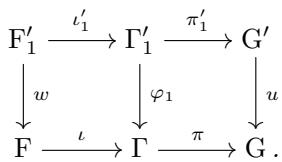
\includegraphics[keepaspectratio]{images/part002_e5b6b945.jpg}}

则存在唯一的群同态 \(\psi : \Gamma_1' \to \Gamma'\)，使得图

\pandocbounded{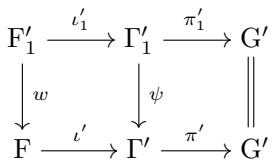
\includegraphics[keepaspectratio]{images/part002_7bcd6e81.jpg}}

交换且 \(\varphi_{1} = \varphi \circ \psi\)。

若群同态 \(\psi : \Gamma_1' \to \Gamma'\) 具有所要的性质，则它满足关系

\[
\psi (\gamma) = (\varphi \circ \psi (\gamma), \pi^ {\prime} \circ \psi (\gamma)) = (\varphi_ {1} (\gamma), \pi_ {1} ^ {\prime} (\gamma))
\]

（对每个 \(\gamma \in \Gamma_1'\)）。反之，从 \(\Gamma_1'\) 到 \(\Gamma \times G'\) 的由 \(\gamma \mapsto (\varphi_1(\gamma), \pi_1'(\gamma))\) 定义的群同态取值在纤维积 \(\Gamma \times_G G'\) 中，因为 \(\pi \circ \varphi_1(\gamma) = u \circ \pi_1'(\gamma)\)（对每个 \(\gamma \in \Gamma_1'\)）。

推论 1. —— 设 \(E_{1}\) 与 \(E_{2}\) 是 G 被 F 的 \(\tau\)-扩张，并设 \(\psi\) 是一个 \(\tau\)-扩张的态射（从 \(E_{1}\) 到 \(E_{2}\) 的）。用 \(\varphi_{1}\)（相应地，\(\varphi_{2}\)）表示 \(u^{*}(\mathcal{E}_{1})\)（相应地，\(u^{*}(\mathcal{E}_{2})\)）的典范同态。则存在唯一的 \(\tau'\)-扩张的态射（从 \(u^{*}(\mathcal{E}_{1})\) 到 \(u^{*}(\mathcal{E}_{2})\) 的），记作 \(u^{*}(\psi)\)，使得 \(\varphi_{2} \circ u^{*}(\psi) = \psi \circ \varphi_{1}\)。

只需对 \(\psi \circ \varphi_{1}\) 应用命题 1。

于是 \(\tau^{\prime}\)-扩张 \(u^{*}(\mathcal{E})\) 的类只依赖于 E 的类。我们也用 \(u^{*}:\operatorname{Ex}_{\tau}(\mathrm{G},\mathrm{F})\to\operatorname{Ex}_{\tau^{\prime}}(\mathrm{G}^{\prime},\mathrm{F})\) 表示把一个 \(\tau\)-扩张 E 的类映到 \(\tau^{\prime}\)-扩张 \(u^{*}(\mathcal{E})\) 的类的映射。

推论 2. —— 设 \(u': G'' \to G'\) 是一个群同态，\(\mathcal{E}\) 是 G 被 F 的一个 \(\tau\)-扩张。设 \(\tau'' = \tau' \circ u'\)，并用 \(\varphi\)（相应地，\(\varphi', \varphi''\)）表示与 \(\tau'\)-扩张 \(u^*(\mathcal{E})\)（相应地，\(\tau''\)-扩张 \(u'^*(u^*(\mathcal{E}))\)、\(\tau''\)-扩张 \((u \circ u')^*(\mathcal{E})\)）相伴的典范同态。则存在唯一的态射 \(\psi\)（从 \(\tau''\)-扩张 \(u'^*(u^*(\mathcal{E}))\) 到 \(\tau''\)-扩张 \((u \circ u')^*(\mathcal{E})\) 的），使得 \(\varphi'' \circ \psi = \varphi \circ \varphi'\)。

例. —— 设 H 是 G 的一个子群，\(j : H \to G\) 是典范单射。则对每个 \(\tau\)-扩张 \(\mathcal{E} = (\Gamma, \iota, \pi)\)，\(\tau \circ j\)-扩张 \(j^{*}(\mathcal{E})\) 同构于 \((\bar{\pi}^{1}(H), \iota', \pi')\)，其中 \(\iota' : F \to \bar{\pi}^{1}(H)\)（相应地，\(\pi' : \bar{\pi}^{1}(H) \to H\)）是群同态 \(f \mapsto \iota(f)\)（相应地，\(\gamma \mapsto \pi(\gamma)\)）。更一般地，若群同态 \(u : G' \to G\) 是单射的，则典范同态 \(\varphi\) 是单射的，其像为 \(\bar{\pi}^{1}(u(G'))\)。
